\documentclass[american,]{article}
\usepackage{lmodern}
\usepackage{amssymb,amsmath,amsthm}
\usepackage{ifxetex,ifluatex}
\usepackage{fixltx2e} % provides \textsubscript
\ifnum 0\ifxetex 1\fi\ifluatex 1\fi=0 % if pdftex
  \usepackage[T1]{fontenc}
  \usepackage[utf8]{inputenc}
\else % if luatex or xelatex
  \ifxetex
    \usepackage{mathspec}
  \else
    \usepackage{fontspec}
  \fi
  \defaultfontfeatures{Ligatures=TeX,Scale=MatchLowercase}
\fi
% use upquote if available, for straight quotes in verbatim environments
\IfFileExists{upquote.sty}{\usepackage{upquote}}{}
% use microtype if available
\IfFileExists{microtype.sty}{%
\usepackage{microtype}
\UseMicrotypeSet[protrusion]{basicmath} % disable protrusion for tt fonts
}{}
\usepackage[margin=1in]{geometry}
\usepackage{hyperref}
\hypersetup{unicode=true,
            pdftitle={Improving Convergence Diagnostics for Iterative Simulation},
            pdfauthor={Aki Vehtari, Andrew Gelman, Daniel Simpson, Bob Carpenter, Paul-Christian Bürkner},
            pdfkeywords={keywords},
            pdfborder={0 0 0},
            breaklinks=true}
\urlstyle{same}  % don't use monospace font for urls
\ifnum 0\ifxetex 1\fi\ifluatex 1\fi=0 % if pdftex
  \usepackage[shorthands=off,main=american]{babel}
\else
  \usepackage{polyglossia}
  \setmainlanguage[variant=american]{english}
\fi
\usepackage{natbib}
\bibliographystyle{plainnat}
\usepackage{placeins}
\usepackage{graphicx,grffile}
\makeatletter
\def\maxwidth{\ifdim\Gin@nat@width>\linewidth\linewidth\else\Gin@nat@width\fi}
\def\maxheight{\ifdim\Gin@nat@height>\textheight\textheight\else\Gin@nat@height\fi}
\makeatother
% Scale images if necessary, so that they will not overflow the page
% margins by default, and it is still possible to overwrite the defaults
% using explicit options in \includegraphics[width, height, ...]{}
\setkeys{Gin}{width=\maxwidth,height=\maxheight,keepaspectratio}
\IfFileExists{parskip.sty}{%
\usepackage{parskip}
}{% else
\setlength{\parindent}{0pt}
\setlength{\parskip}{6pt plus 2pt minus 1pt}
}
\setlength{\emergencystretch}{3em}  % prevent overfull lines
\providecommand{\tightlist}{%
  \setlength{\itemsep}{0pt}\setlength{\parskip}{0pt}}
\setcounter{secnumdepth}{3}
% Redefines (sub)paragraphs to behave more like sections
\ifx\paragraph\undefined\else
\let\oldparagraph\paragraph
\renewcommand{\paragraph}[1]{\oldparagraph{#1}\mbox{}}
\fi
\ifx\subparagraph\undefined\else
\let\oldsubparagraph\subparagraph
\renewcommand{\subparagraph}[1]{\oldsubparagraph{#1}\mbox{}}
\fi

%%% Use protect on footnotes to avoid problems with footnotes in titles
\let\rmarkdownfootnote\footnote%
\def\footnote{\protect\rmarkdownfootnote}

%%% Change title format to be more compact
\usepackage{titling}

% Create subtitle command for use in maketitle
\newcommand{\subtitle}[1]{
  \posttitle{
    \begin{center}\large#1\end{center}
    }
}

\setlength{\droptitle}{-2em}

   
\usepackage{booktabs}
\usepackage{longtable}
\usepackage{array}
\usepackage{multirow}
\usepackage[table]{xcolor}
\usepackage{wrapfig}
\usepackage{float}
\usepackage{colortbl}
\usepackage{pdflscape}
\usepackage{tabu}
\usepackage{threeparttable}
\usepackage{threeparttablex}
\usepackage[normalem]{ulem}
\usepackage{makecell}

\usepackage{mathtools}
\usepackage[utf8]{inputenc}
\usepackage[T1]{fontenc}
\usepackage{textcomp}
\usepackage{graphicx,pdflscape}
\usepackage{geometry}
\usepackage{amsmath}
\usepackage{float}
\usepackage{supertabular}
\usepackage{booktabs,caption,fixltx2e}
\usepackage{tcolorbox}
\usepackage{paralist}
\usepackage{multicol}
\setcitestyle{round}
\newcommand\numberthis{\addtocounter{equation}{1}\tag{\theequation}}
\DeclareMathOperator*{\dd}{d}
\DeclareMathOperator{\Cauchy}{Cauchy}
\DeclareMathOperator{\N}{N}
\DeclareMathOperator{\Gam}{Gamma}
\newcommand{\Rhat}{$\widehat{R}$}
\newcommand{\sRhat}{split-$\widehat{R}$}
\theoremstyle{definition}
\newtheorem{example}{Example}

 \title{Rank-normalization, folding, and localization: A version of $\widehat{R}$ that successfully assesses the convergence of iterative simulation algorithms}
    \pretitle{\vspace{\droptitle}\centering\huge}
  \posttitle{\par}
    \author{Aki Vehtari, Andrew Gelman, Daniel Simpson, Bob Carpenter, Paul-Christian Bürkner}
    
    \author{
Aki Vehtari\footnote{Helsinki Institute for Information Technology HIIT,
  Department of Computer Science, Aalto University, Finland.},
   Andrew Gelman\footnote{Department of Statistics, Columbia University, New York.},
 Daniel Simpson\footnote{Department of Statistical Sciences, University of Toronto, Canada.},
 Bob Carpenter$^{\dagger}$,
and Paul-Christian B\"{u}rkner\footnote{Department of Psychology, University of M\"{u}nster, Germany}
}
    
    \preauthor{\centering\large\emph}
  \postauthor{\par}
%    \date{4 March 2019}
%    \predate{}\postdate{}


\begin{document}
\maketitle
\begin{abstract}
  Markov chain Monte Carlo is the main computational tool for Bayesian 
  statistics, however it is known that we must carefully monitor the
  convergence behaviour of the chain lest poor computation bias our estimates.
In this paper we show that the most commonly used convergence diagnostic \Rhat\ 
of \citet{Gelman+Rubin:1992} has serious flaws and we
propose an alternative that fixes them. We also introduce
  a collection of quantile based local efficiency
  measures, and a practical approach for computing Monte Carlo error
  estimates for quantiles. We suggest that common trace plots should
  be replaced with rank plots from multiple chains. Finally, we give
  concrete recommendations for how these methods should be used
  in practice.
\end{abstract}

\hypertarget{introduction}{%
\section{Introduction}\label{introduction}}

 Markov chain Monte Carlo (MCMC) methods form the core
of many methods in computational statistics, especially 
in Bayesian applications where the goal is to represent
posterior inference using a sample of posterior draws. While MCMC, 
as well as more general iterative
simulation algorithms, can usually be proven to converge
to the target distribution as the number of draws approaches infinity,
there are rarely strong guarantees about their behaviour after a 
finite number of draws. In fact, decades of experience tell us that
the finite sample behaviour of these algorithms can be almost arbitrarily bad.


In an attempt to assuage our fear that our MCMC algorithm may
not have converged, we typically run multiple 
independent chains  to see if the obtained 
distribution is similar across chains.  We typically also visually inspect
the sample path of the chains as well as some summary statistics such as
investigating the empirical autocorrelation function. 

Running multiple chains is critical to any MCMC convergence diagnostic. Figure
\ref{converge.challenge} illustrates two ways in which sequences of
iterative simulations can fail to converge.  In the first example, two chains
are in different parts of the target distribution, in the second
example, the chains move but have not attained stationarity. Slow mixing can arise with multimodal target distributions or when a chain is
stuck in a region of high curvature with a step size too large to make an
acceptable proposal for the next step. The two examples in Figure \ref{converge.challenge}  make it clear that 
any method for assessing mixing and effective sample size should use information
between and within chains.

\begin{figure}
  \center
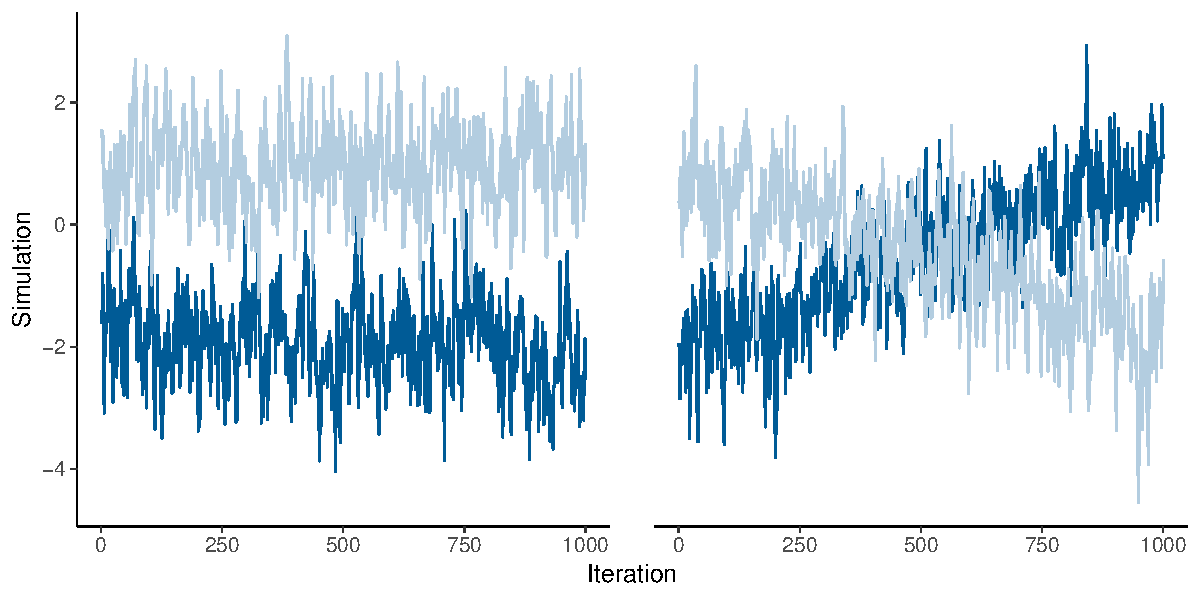
\includegraphics[width=0.7\textwidth]{graphics/convergechallenge.pdf}
\caption{ Examples of two challenges in assessing convergence of iterative
simulations. (a) In the left plot, either sequence alone looks stable, but the
juxtaposition makes it clear that they have not converged to a common
distribution. (b) In the right plot, the two sequences happen to cover a common
distribution but neither sequence appears stationary. These graphs demonstrate
the need to use between-sequence and also within-sequence information when
assessing convergence. Adapted from \citet{BDA3}).}
\label{converge.challenge}
\end{figure}

As we are often fitting models with large
numbers of parameters, it is not realistic to expect to make and interpret
trace plots such as in Figure \ref{converge.challenge} for all
quantities of interest. Hence we need numerical summaries that can flag
potential problems. 


Probably the most widely-used attempt to construct a more formally justified 
convergence diagnostic  is the  \(\widehat{R}\) statistic
\citep{Gelman+Rubin:1992, Brooks+Gelman:1998} and
split-\(\widehat{R}\) \citep{BDA3}.  These quantities monitor the ratio of
the within-chain marginal variances and the between-chain marginal variances
of the simulations. The idea is that if a chain has not converged to 
stationarity, these quantities will be quite different.  The difference between
the original $\widehat{R}$ and split-$\widehat{R}$ is that the latter also compares 
the marginal distributions of the first half of each chain with the second
half of each chain, to try to ensure that each chain has itself converged.  In this
paper we will only consider \sRhat .

The \sRhat\ is most effective if it is computed using multiple chains initialized at a 
diverse set of starting points. This is to reduce the dependence of diagnostic
on the starting point of the chain and reduce the chance that we falsely diagnose
the chain as converging when beginning at a different point would lead to a 
qualitatively different posterior.

In the context of Markov chain Monte Carlo, one can interpret \sRhat\ 
with diverse seeding as an operationalization of the qualitative statement 
that the convergence of the Markov chain is relatively insensitive to the starting 
point (at least within a 
reasonable part of the parameter space). This is the closest we can come to 
verifying empirically that the Markov chain is geometrically ergodic, which is a critical 
property if we want  a central limit theorem to hold for the approximate
posterior expectations. Without this, we have no control over the large
deviation behaviour of the estimates and the constructed Markov chains will
be useless for practical purposes.

 
The problem is that \Rhat\ and \sRhat\ do not reliably work when analyzing 
generic iterative algorithms.  This is particularly a problem when we use them 
within generic software packages like \texttt{Stan} \citep{Stan:JSS:2017} or 
analysis tools like the \texttt{coda} package \citep{coda2006} of the 
programming language R \citep{R2018}. The following example shows how the 
failure occurs.

\begin{figure}
\centering
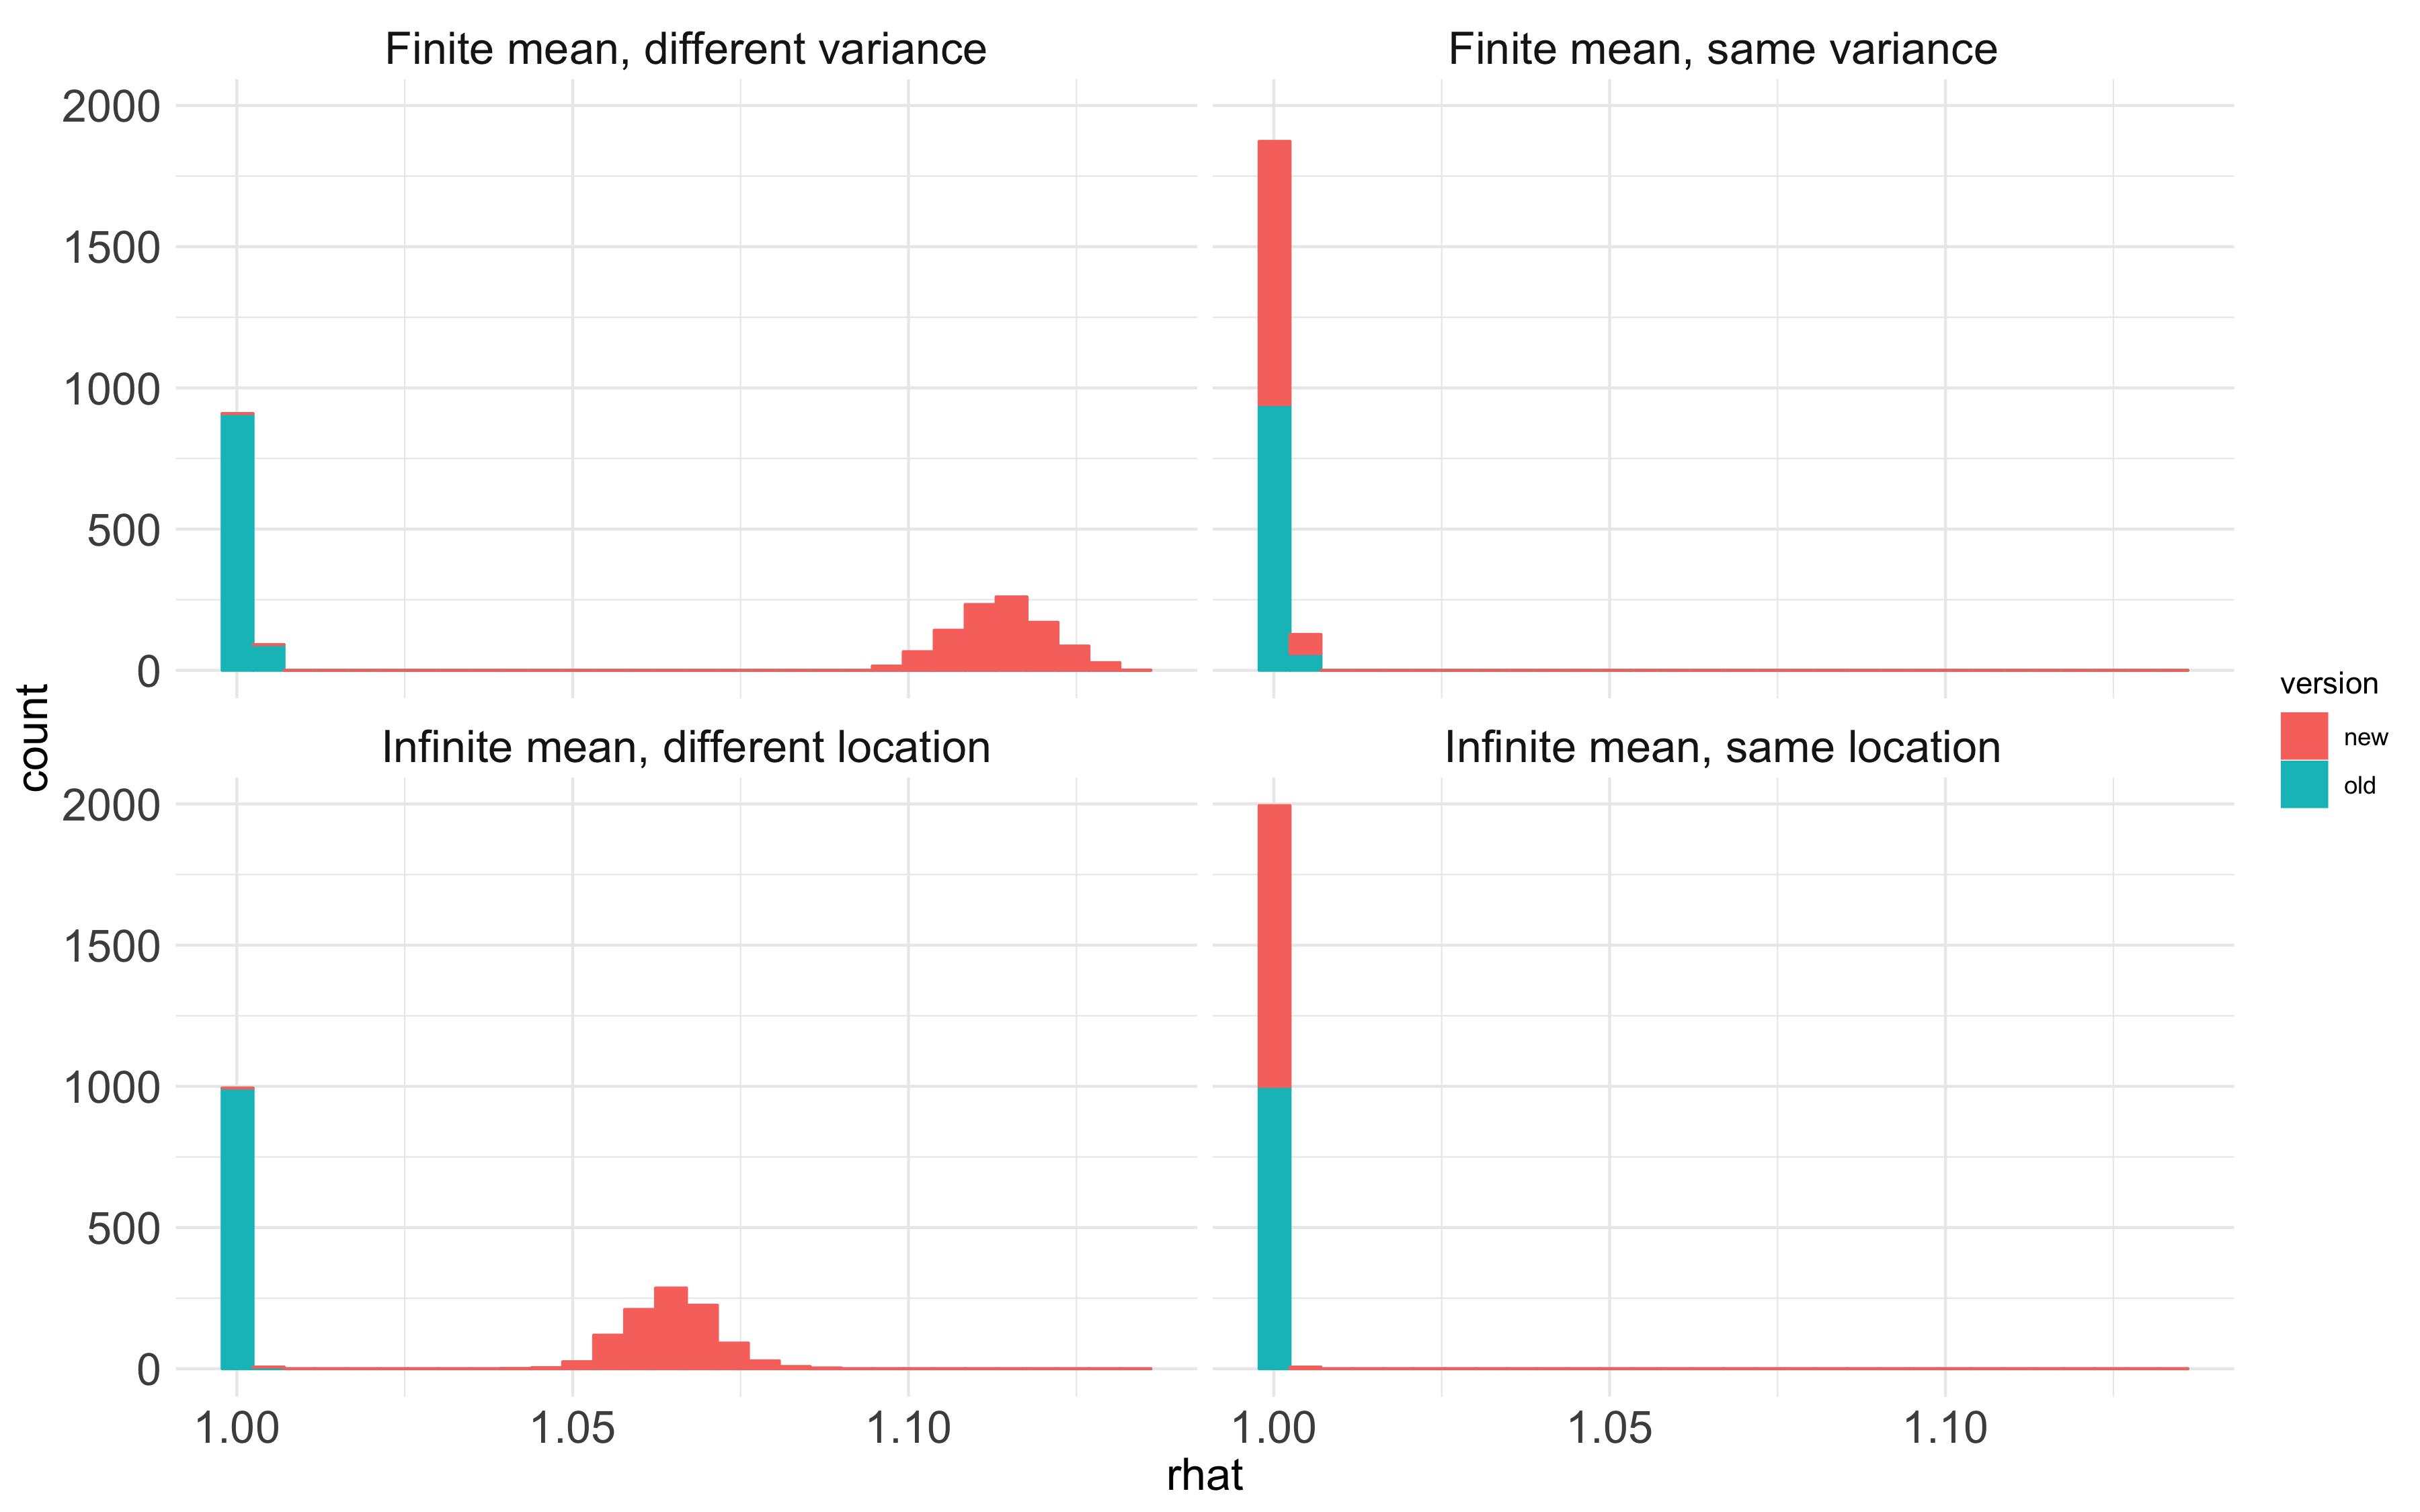
\includegraphics[width=\textwidth]{graphics/simple_rhat_compare.png}
\caption{  The synthetic problem described in Example 1 demonstrates
two modes of failure for the existing \sRhat\ estimator. Each plot shows
histograms of \sRhat\ values over $1000$ replications of four chains each
with a thousand draws. In the left column, one of these four chains was 
incorrect. In the top left plot, one of the four chains had a variance that was too low.
In the bottom left plot, one of the four chains was systematically biased. 
In both cases, the traditional \sRhat\ estimate does not detect the poor
behaviour, while the new value does. In the right column, all the chains are
simulated with the same distribution. The chains used for the top row plots target 
a normal distribution, while the chains used for the bottom row plots target
a Cauchy distribution. \label{fig:simple_example}}
\end{figure}

\medskip
\begin{example}
Figure~\ref{fig:simple_example} shows the distribution of \sRhat\  values over $1000$ replications for four different scenarios where four chains are run for $1000$ iterations. The chains on the top row are independent AR(1) processes with autoregressive parameter $\rho=0.3$. The figure in the top left column reports the distribution of the \sRhat\ statistics  when the variance of one of the four chains is $1/3$ of the variance of the others. This corresponds to a scenario where one chain fails to correctly explore the parameter space. The \sRhat\ statistic defined in \citet{BDA3}  does not detect the poor mixing, while the new variant of \sRhat\ defined later in this paper does. The second column of the top row is the same scenario but with all the chains having the same variance and both \sRhat\ values correctly identify that mixing occurs.

The second row of Figure~\ref{fig:simple_example} shows the behaviour of \sRhat\ when the target distribution has infinite variance. In this case the chains were constructed as a ratio of stationary AR(1) processes with autoregressive parameter  $\rho=0.3$, which makes the target distribution Cauchy.  All of the simulated chains have  unit scale parameter, but in the left hand column one of the four chains is shifted two  units to the right.  Whereas the \citet{BDA3} version of \sRhat\ would catch this behavior if the chain had finite variance, we can see here that it incorrectly returns a value very close to one. On the other hand, our new \sRhat\ statistic correctly catches the error. The bottom right column shows that both version of \sRhat\ work when the four chains have the same distribution. 
\end{example}

This example identifies two problems with \sRhat : 
\begin{enumerate}
\item If the chains have different variances but the same mean parameters, $\widehat{R} \approx 1$.
\item If the chains don't have finite variance, $\widehat{R} \approx 1$ even if one of the chains has a different location parameter to the others. This can also lead to numerical instability for thick-tailed distributions even if they technically have a finite (but large) variance. We note that it's typically very hard to assess empirically
if a chain has large but finite variance or infinite variance.
\end{enumerate}

Another problem is that split-\(\widehat{R}\) is
usually computed only for the posterior mean. While this provides an estimate 
for the convergence in the bulk of the distribution, it says little about the 
convergence in the tails, which is a concern for posterior 
interval estimates as well as for inferences about rare events.

All of these observations lead to the conclusion that the \Rhat\ statistic 
as it is currently defined is not a good measure of convergence. However, it is 
easy to compute and sensitive to certain types of non-convergence. So, 
in this paper, we propose improvements of \sRhat\ that overcome the  
problems described above. Furthermore, as the convergence
of the Markov chain need not be uniform across the parameter space, we
propose a localized version of \sRhat\ and corresponding efficiency measures 
that allow us to assess better the behaviour of localized 
functionals of the chain. Finally, we propose three new methods to visualize the 
convergence of an iterative algorithm that are more informative than standard 
trace plots.

The remainder of this paper is organized as follows. 
For readers primarily interested in applying our newly proposed convergence 
diagnostics, we first provide practical recommendations about their usage
that do not require detailed understanding of the underlying mathematics.
We continue by reviewing the standard 
\sRhat\, before proposing improvements that repair the problems noted above. 
We then propose some localized diagnostics and some new diagnostic plots. 
Finally, we show the behavior of the new diagnostics on a variety of examples.
In the appendix, we provide mathematical details about effective sample size 
calculations and present more numerical experiments. All computer code and an 
even larger variety of numerical experiments are available in the online 
appendix (\url{https://avehtari.github.io/rhat_ess/rhat_ess.html}).



\section{Recommendations for practice}
In this section we lay out our specific recommendations for using the tools 
developed in this paper in practice. In the interest of specificity, we have 
provided numerical targets for both \Rhat\ and the Effective Sample Size (ESS). 
However, these values should be adapted as necessary for the given application.

In Section \ref{improving-convergence-diagnostics}, we propose modifications to the 
standard \Rhat\ estimator based on rank-normalizing (Section 
\ref{rank-normalization}) and folding (Section
 \ref{diagnostics-for-folded-draws}) the posterior draws.
These allow us to produce a single number summary  that demonstrates how
 robust estimators of the location and scale of the target distribution differs
 between chains.  For simplicity, we still write this as \Rhat .
 
Roughly speaking, the ESS of a quantity of interest captures how many 
independent samples contain the same amount of information as the dependent 
samples obtained by the MCMC algorithm. Clearly, the higher the ESS the better.
When there might be difficulties with mixing, it is important to use between-chain 
information in computing the ESS. For instance, in the sorts of
funnel-shaped distributions that arise with hierarchical models, differences 
in step size adaptation can lead to chains to have
different behavior reaching the narrow part of the funnel. For multimodal 
distributions with well-separated modes, the split-\(\widehat{R}\)
adjustment of the ESS leads to an ESS estimate that is close to the number of
distinct modes that are found (i.e., very small). 
In this situation, ESS computed on from a single chain will most likely 
overestimate the ESS. The robustness of a split-\(\widehat{R}\) adjusted
ESS can be improved by running more chains and we recommend running at least 
four chains by default and only using the samples if  $\widehat{R} < 1.01$. 
This is a much tighter threshold than the one recommended by 
\citet{Gelman+Rubin:1992}, reflecting lessons learnt over more than 25 years of use.

As \citet{vats2018revisiting} note, a small value of \Rhat\ is not enough to ensure 
that an MCMC procedure is useful in practice. It also needs to have a sufficiently
large number of effective samples. Rather than reducing the threshold for \Rhat\
to indirectly ensure the number of effective samples, we recommend monitoring
the ESS directly. As with the value of \Rhat, we 
recommend computing the ESS on the rank-normalized samples. This does not
directly compute the ESS relevant for computing the mean of the parameter, but 
instead computes a quantity that is well defined even if the chains do not 
have finite mean or variance.  Specifically, it computes the ESS of samples 
from a \emph{normalized} version of the parameter, that is the parameter 
transformed to normality. This is still indicative of the number of effective 
samples for computing means and, in particular, if it is low the computed
expectations are unlikely to be good approximations to the actual
target expectations.  We recommend requiring that the rank-normalized ESS is 
 greater than $400$. When running four chains, this corresponds to having
a rank-normalized effective sample size of at least 50 per split chain.

Only when the rank-normalized and folded \Rhat\ values are less than the
prescribed threshold and the rank-normalized ESS is greater than $400$ do we recommend
computing the actual (i.e., not rank-normalized) effective sample size for the 
quantity of interest. This can then be used to assess the MCSE for the quantity
of interest. Application specific information is needed to 
assess if the MCSE is small enough to answer the question at hand.

Finally, if you plan to report quantile estimates or credible intervals, we 
strongly suggest assessing the convergence of the chains for these quantiles.
In Section \ref{convergence-diagnostics-for-quantiles} we show that
convergence of Markov chains is not uniform across the parameter space
and propose diagnostics and effective sample sizes specifically for extreme 
quantiles. This is \emph{different} from the standard ESS estimate (which 
we refer to as the ``bulk-ESS``), which mainly assesses how well
the centre of the distribution is resolved. Instead, these ``tail-ESS`` 
measures allow the user to estimate the MCSE for interval estimates.


\hypertarget{SplitRhat}{%
\section{Split-$\widehat{R}$ and the effective sample size}\label{SplitRhat}}

When coupled with an ESS estimate, the  \sRhat\ is the most common way to
assess whether an MCMC algorithm has converged.  While there is a link between
these two measures  for a single chain \citep{vats2018revisiting}, we prefer to 
treat them as two separate questions: ``Did the chain converge?'' (\sRhat) and 
``Do we have enough samples?'' (ESS).  In this section we define the \sRhat\ 
statistic that we propose to modify. 
The definition of the ESS as used in the present paper is given in Appendix~A.
We will refer to this particular ESS measure as \(S_{\rm eff}\).

The original \(\widehat{R}\) statistic
\citep{Gelman+Rubin:1992, Brooks+Gelman:1998} and
split-\(\widehat{R}\) \citep{BDA3} are both based on the ratio of
between and within-chain marginal variances of the simulations, while
the latter is computed from split chains (hence the name).

Here we present split-\(\widehat{R}\),
following \citet{BDA3}, but using the notation of
\citet{StanBook}. This implementation represents the current 
standard in convergence diagnostics for iterative simulations. In the
equations below, \(N\) is the number of draws per chain, \(M\) is the
number of chains, and \(S=MN\) is the total number of draws from all
chains. For each scalar summary of interest \(\theta,\) we compute \(B\)
and \(W,\) the between- and within-chain variances:

\begin{align}
B &= \frac{N}{M-1}\sum_{m=1}^{M}(\overline{\theta}^{(.m)} - 
\overline{\theta}^{(..)})^2, \quad \mbox{where} \quad 
\overline{\theta}^{(.m)}=\frac{1}{N}\sum_{n=1}^N \theta^{(nm)}, \quad
\overline{\theta}^{(..)} = \frac{1}{M}\sum_{m=1}^M\overline{\theta}^{(.m)} 
\\
W &= \frac{1}{M}\sum_{m=1}^{M}s_j^2, \quad \mbox{where} \quad
s_m^2=\frac{1}{N-1} \sum_{n=1}^N (\theta^{(nm)}-\overline{\theta}^{(.m)})^2.
\end{align}

The between-chain variance, \(B\), also contains the factor \(N\)
because it is based on the variance of the within-chain means,
\(\overline{\theta}^{(.m)},\) each of which is an average of \(N\)
values \(\theta^{(nm)}\). We can estimate \(\mbox{var}(\theta | y)\),
the marginal posterior variance of the estimand, by a weighted average
of \(W\) and \(B\), namely,
\begin{equation}
\widehat{\mbox{var}}^+(\theta| y) = \frac{N-1}{N}W + \frac{1}{N}B.
\end{equation}

This quantity \emph{overestimates} the marginal posterior variance
assuming the starting distribution of the simulations is appropriately
overdispersed compared to the target distribution, but is
\emph{unbiased} under stationarity (that is, if the starting
distribution equals the target distribution), or in the limit
\(N\rightarrow\infty\). To have an overdispersed starting distribution,
independent Markov chains should be initialized with diffuse starting
values for the parameters. 

Meanwhile, for any finite \(N\), the within-chain variance \(W\) should
\emph{underestimate} \(\mbox{var}(\theta |y)\) because the
individual chains haven't had the time to explore all of the target
distribution and, as a result, will have less variability. In the limit
as \(N\rightarrow\infty\), the expectation of \(W\) also approaches
\(\mbox{var}(\theta |y)\). \citet{vats2018revisiting} propose a different variance estimator that is more efficient for single chains, however we are willing to trade off a slightly higher variance for the increase diagnostic sensitivity (described in the Introduction) that running multiple chains brings.

We monitor convergence of the iterative simulations to the target
distribution by estimating the factor by which the scale of the current
distribution for \(\theta\) might be reduced if the simulations were
continued in the limit \(N\rightarrow\infty\). This potential scale
reduction is estimated as,
\begin{equation}
\widehat{R} = \sqrt{\frac{\widehat{\mbox{var}}^+(\theta | y)}{W}},
\end{equation}
which for an ergodic process declines to 1 as \(N\rightarrow\infty\). We call this
split-\(\widehat{R}\) because we are applying it to chains that
have been split in half so that \(M\) is twice the number of actual
chains. Without splitting, \(\widehat{R}\) would get fooled by
non-stationary chains as in Figure \ref{converge.challenge}b.

The value of \Rhat\ requires reliable estimates of variances and autocorrelations, which can
only occur if the chain has enough independent replicates in it. In particular, we only recommend 
relying on the \Rhat\ estimate to make decisions about the quality of the chain if each of the 
split chains has an ESS estimate of at least 50. In the our minimum recommended setup of four
parallel chains, the total ESS should be at least 400 before we expect the \Rhat value to be useful.


\hypertarget{improving-convergence-diagnostics}{%
\section{Improving convergence
diagnostics}\label{improving-convergence-diagnostics}}

\hypertarget{rank-normalization}{%
\subsection{Rank normalization helps  \Rhat\ when there are heavy tails}\label{rank-normalization}}

As split-\(\widehat{R}\) and \(S_{\rm eff}\) are well defined
only if the marginal posteriors have finite mean and variance, we
propose to use rank normalized parameter values instead of the actual
parameter values for the purpose of diagnosing convergence.

Rank normalized split-\(\widehat{R}\) and \(S_{\rm eff}\) are
computed using the equations in Section \ref{SplitRhat} and Appendix~A, but
replacing the original parameter values \(\theta^{(nm)}\) with their
corresponding rank normalized values denoted as \(z^{(nm)}\). Rank
normalization is done a follows: First, replace each value
\(\theta^{(nm)}\) by its rank \(r^{(nm)}\) within the pooled draws from all chains.
 Average rank for ties are
used to conserve the number of unique values of discrete quantities.
 Second, normalize ranks via the inverse normal transformation,
\begin{equation}
z^{(nm)} = \Phi^{-1}((r^{(nm)}-0.5)/S).
\end{equation}

For continuous variables and \(S \rightarrow \infty\), the rank
normalized values are normally distributed. Using normalized ranks
\(z^{(nm)}\) instead of ranks \(r^{(nm)}\) themselves has the additional
benefit that the behavior of \(\widehat{R}\) and \(S_{\rm eff}\) do
not change for normally distributed parameters.  Furthermore, rank-normalized \Rhat\ and \(S_{\rm eff}\) are invariant to univariate transformations. Hence    
rank-normalized \Rhat\ and \(S_{\rm eff}\) are approximations to the ordinary \Rhat\ and \(S_{\rm eff}\) for a nice transformation of the parameter of interest.
The effects of rank normalization are further explored in the online appendix.

We will use the term \emph{bulk effective sample size} (bulk-ESS or
bulk-\(S_{\rm eff}\)) to refer to the effective sample size based on the
rank normalized draws. Bulk-ESS is useful for diagnosing problems due to
trends or different locations of the chains (see Appendix~B). Further, it is
well defined even for distributions with infinite mean or variance, a
case where previous ESS estimates fail. However, due to the rank
normalization, Bulk-ESS is no longer directly applicable to estimate the
Monte Carlo standard error of the posterior mean. We will come back to
the issue of computing Monte Carlo standard errors for relevant
quantities in Section \ref{mcse}.

\hypertarget{diagnostics-for-folded-draws}{%
\subsection{Folding chains detects errors in variance and trouble exploring the tails}\label{diagnostics-for-folded-draws}}


Both original and rank normalized split-\(\widehat{R}\) can be
fooled if the chains have the same location but different scales. This
can happen if one or more chains is stuck near the middle of the distribution. 
To alleviate this problem, we propose a
rank normalized split-\(\widehat{R}\) statistic not only for the
original draws \(\theta^{(nm)}\), but also for the corresponding {\em folded}
draws \(\zeta^{(mn)}\), absolute deviations from the median,
\begin{equation}
\label{zeta}
\zeta^{(mn)} = \left|\theta^{(nm)}-{\rm median}(\theta)\right|.
\end{equation}

We call the rank normalized split-\(\widehat{R}\) measure computed on the
 \(\zeta^{(mn)}\) values  \emph{folded-split}-\(\widehat{R}\).
  This measures convergence in the
tails rather than in the bulk of the distribution. To obtain a single
conservative \(\widehat{R}\) estimate, we propose to report the maximum
of rank normalized split-\(\widehat{R}\) and rank normalized
folded-split-\(\widehat{R}\) for each parameter.

\hypertarget{convergence-diagnostics-for-quantiles}{%
\subsection{Localizing convergence diagnostics: assessing the quality of quantiles, the median absolute deviation, and small-interval probabilities }\label{convergence-diagnostics-for-quantiles}}

The new \(\widehat{R}\) and bulk-ESS introduced above are useful as overall efficiency
measures. Next we introduce
convergence diagnostics for quantiles and related quantities, which are more focused measures and help to diagnose reliability of  reported
posterior intervals. Estimating
the efficiency of quantile estimates has a high practical
relevance in particular as we observe the efficiency for tail quantiles
to often be lower than for the mean or median.  This especially has implications
if people are making decisions based on whether or not a specific quantile
is below or above a fixed value (for example, if a credible interval contains zero).

The \(\alpha\)-quantile
is defined as the parameter value \(\theta_\alpha\) for which
\(p(\theta \leq \theta_\alpha) = \alpha\). An estimate
\(\hat{\theta}_\alpha\) of \(\theta_\alpha\) can thus be obtained by
finding the \(\alpha\)-quantile of the empirical cumulative distribution function (ECDF) of the
posterior draws \(\theta^{(s)}\). However, quantiles cannot be written
as an expectation, and thus the above equations for \(\widehat{R}\) and
\(S_{\rm eff}\) are not directly applicable. Thus, we first focus on the
efficiency estimate for the cumulative probability
\(p(\theta \leq \theta_\alpha)\) for different values of
\(\theta_\alpha\).

For any \(\theta_\alpha\), the ECDF gives an estimate of the cumulative
probability,
\begin{equation}
p(\theta \leq \theta_\alpha) \approx \bar{I}_\alpha = \frac{1}{S}\sum_{s=1}^S
I(\theta^{(s)} \leq\theta_\alpha),
\end{equation}
where \(I(\cdot)\) is the indicator function. The indicator function
transforms simulation draws to 0's and 1's, and thus the subsequent
computations are bijectively invariant. Efficiency estimates of the ECDF
at any \(\theta_\alpha\) can now be obtained by applying
rank-normalizing and subsequent computations directly on the indicator
function's results.

Assuming that we know the CDF to be a certain continuous function \(F\)
which is smooth near an \(\alpha\)-quantile of interest, we could use
the delta method to compute a variance estimate for
\(F^{-1}(\bar{I}_\alpha)\). Although we don't usually know \(F\), the
delta method approach reveals that the variance of \(\bar{I}_\alpha\)
for some \(\theta_\alpha\) is scaled by the (usually unknown) density
\(f(\theta_\alpha)\), but the efficiency depends only on the ratio of variances, which means that the efficiency of \(F^{-1}(\bar{I}_\alpha)\) is well approximated asymptotically by the  efficiency
of \(\bar{I}_\alpha\). Thus, we can use the effective sample size for
the ECDF (computed using the indicator function
\(I(\theta^{(s)} \leq \theta_\alpha)\)) also for the corresponding
quantile estimates. More details on the variance of the cumulative
distribution function can be found in the online appendix.

To get a better sense of the sampling efficiency in the
distributions' tails, we propose to compute the minimum of the effective
sample sizes of the 5\% and 95\% quantiles, which we will call
\emph{tail effective sample size} (tail-ESS or tail-\(S_{\rm eff}\)).
Tail-ESS can help diagnosing problems due to different scales of the
chains (see Appendix~B).


Since the marginal posterior distributions might not have finite mean
and variance, by default \texttt{rstan} \citep{RStan.2.17} and \texttt{rstanarm}
\citep{RStanARM.2.17} report median and median absolute deviation (MAD)
instead of mean and standard error. Median and MAD are well defined
even when the marginal distribution does not have finite mean and
variance. Since the median is just the 50\% quantile, we can get an
efficiency estimate for it as for any other quantile.

Further, we can also compute an efficiency estimate for the median
absolute deviation by computing the efficiency estimate of an
indicator function based on the folded parameter values \(\zeta\) (see
Equation (\ref{zeta})):
\begin{equation}
p(\zeta \leq \zeta_{0.5}) \approx \bar{I}_{\zeta,0.5} = \frac{1}{S}\sum_{s=1}^S
I(\zeta^{(s)} \leq \zeta_{0.5}),
\end{equation}
where \(\zeta_{0.5}\) is the median of the folded values. The efficiency estimate for the MAD is obtained by applying the same
approach as for the median (and other quantiles) but with the folded
parameters values.


We can get more local efficiency estimates by considering small
probability intervals. We propose to compute the efficiency estimates
for
\begin{equation}
\bar{I}_{\alpha,\delta} = p(\hat{Q}_\alpha < \theta \leq \hat{Q}_{\alpha+\delta}),
\end{equation}

where \(\hat{Q}_\alpha\) is an empirical \(\alpha\)-quantile,
\(\delta=1/k\) is the length of the interval with some positive integer
\(k\), and \(\alpha \in (0,\delta,\ldots,1-\delta)\) changes in steps of
\(\delta\). Each interval has \(S/k\) draws, and the efficiency measures
the autocorrelation of an indicator function which is \(1\) when the
values are inside the specific interval and \(0\) otherwise. This gives
us a local efficiency measure which does not depend on the shape of the
distribution.

\hypertarget{mcse}{%
\subsection{Monte Carlo error estimates for quantiles}\label{mcse}}

It is common practice to only report the Monte Carlo error of the mean,
but not of quantiles and related quantities. As the delta method for
computing the variance would require explicit knowledge of the
normalized posterior density, which we don't have except in most non-trivial
cases, we propose the following alternative approach to compute Monte
Carlo standard errors of quantiles:

\begin{enumerate}
\def\labelenumi{\arabic{enumi}.}
\item
  Compute quantiles of the beta distribution with shape parameters
  \begin{equation}
  \beta_1 = S_{\rm eff} / S \times \bar{I}_\alpha+1 \quad \text{and} \quad
  \beta_2 = S_{\rm eff} / S \times (1-\bar{I}_\alpha) + 1.
  \end{equation} Including \(S_{\rm eff}/S\) takes into account the
  efficiency of the posterior draws.
\item
  Find indices in \(s \in \{1,\ldots,S\}\) closest to the ranks of these
  quantiles. For example, for quantile \(Q\), find
  \(s = {\rm round(Q \times S)}\).
\item
  Use the corresponding \(\theta^{(s)}\) from the list of sorted
  posterior draws as quantiles from the error distribution. 
\end{enumerate}


\hypertarget{diagnostic-visualizations}{%
\subsection{Diagnostic visualizations}\label{diagnostic-visualizations}}

In order to intuitively grasp convergence of iterative algorithms, we
propose several new diagnostic visualizations in addition to the numerical
convergence diagnostics discussed above. We illustrate the usage of
these visualizations by means of several examples in Section
\ref{examples}.

\hypertarget{rank-plots}{%
\paragraph{Rank plots.}\label{rank-plots}}
Extending the idea of using ranks instead of the original parameter
values, we propose to use rank plots for each chain instead
of trace plots. Rank plots are histograms of the
ranked posterior samples (ranked over all chains) plotted separately for
each chain. If all of the chains are targeting the same posterior, we expect the 
ranks in each chain to be uniform, whereas if one chain has a different location
or scale parameter, this will be reflected in the deviation from uniformity. 
 If rank plots of all chains look similar, this indicates
good mixing of the chains. As compared to trace plots, rank plots don't
tend to squeeze to a fuzzy mess in case of long chains.

\hypertarget{quantile-and-small-interval-plots}{%
\paragraph{Quantile and small interval
plots.}\label{quantile-and-small-interval-plots}}
The efficiency of quantiles or small interval probabilities may vary
drastically across different quantiles and small interval positions,
respectively. We thus propose to use diagnostic plots that display
efficiency of quantiles or small interval probabilities across their
whole range to better diagnose areas of the distributions that the
iterative algorithm fails to explore efficiently.

\hypertarget{efficiency-change-plots}{%
\paragraph{Efficiency per iteration plots.}\label{efficiency-change-plots}}
For a well explored distribution, we expect the ESS measures to grow
linearly with the total number of draws \(S\), or, equivalently, that
the relative efficiency (ESS divided \(S\)) is approximately constant
for different values of \(S\). For small number of draws, both bulk and
tail-ESS may be unreliable and cannot necessarily detect convergence
problems. As a result, some convergence problems may only be
detectable as \(S\) increases, which then implies the ESS to grow slower
then linear or even decrease with increasing \(S\). Equivalently, in
such a case, we would expect to see a relatively sharp drop in the
relative efficiency measures. We therefore propose to plot the change of
both bulk and tail ESS with increasing \(S\). This can be done based on
a single model without a need to refit, as we can just extract initial
sequences of certain length from the original chains. However, it should
be noted that some convergence problems only occur at relatively high
\(S\) and may thus not be detectable if the total number of draws is too
small.

\hypertarget{examples}{%
\section{Examples}\label{examples}}

In this section, we will go through some examples to demonstrate the
usefulness of our proposed methods as well as the associated workflow
for determining convergence. The online appendix contains all model
details, code to reproduce the results and more detailed analysis of
different algorithm variants, and further
examples\footnote{\url{https://avehtari.github.io/rhat_ess/rhat_ess.html}}.

Unless mentioned otherwise, we use dynamic Hamiltonian Monte Carlo with
multinomial sampling \citep{betancourt2017conceptual} as implemented
in Stan \citep{StanManual.2.18.0} and run 4 chains each with 1000
warmup iterations and 1000 post-warmup iterations used for inference.

\hypertarget{cauchy-a-distribution-with-infinite-mean-and-variance}{%
\subsection{Cauchy: A distribution with infinite mean and
variance}\label{cauchy-a-distribution-with-infinite-mean-and-variance}}

The classic split-\(\widehat{R}\) are based on calculating
within and between chain variances. If the marginal distribution of a
chain is such that the variance is not defined (i.e., infinite), the
classic split-\(\widehat{R}\) is not well justified. In this
section, we will use the Cauchy distribution as an example of such a
distribution. 

\hypertarget{nominal-parameterization-of-the-cauchy-distribution}{%
\subsubsection*{Nominal parameterization of the
Cauchy distribution}\label{nominal-parameterization-of-the-cauchy-distribution}}

The nominal Cauchy model with direct parameterization is
\begin{align}
  x \sim \Cauchy(0,1).
\end{align}
We set an independent Cauchy distribution for each element of the 50-dimensional 
real vector $x$. Dynamic HMC specific diagnostics, such as divergent
transitions as well as iterations that exceed the maximum treedepth,
indicate slow mixing of the chains.


Several split-\(\widehat{R}>1.01\) and some ESS \(<400\)
also indicate convergence problems. The online appendix contains more results 
with longer chains and other \(\widehat{R}\) diagnostics.
%
We can further analyze potential problems using local efficiency and
rank plots. We specifically investigate \(x_{36}\), which, in this
specific run, had the smallest tail-ESS of 34. 
Figure~\ref{fig:local-ess-fit-nom-1} shows the local efficiency of small 
interval probability estimates (see Section \ref{convergence-diagnostics-for-quantiles}).
The efficiency of sampling is very low in the tails, which is clearly
caused by slow mixing in long tails of the Cauchy distribution.  
%
Figure~\ref{fig:quantile-ess-fit-nom-1} shows the efficiency
of quantile estimates (see Section \ref{convergence-diagnostics-for-quantiles}), 
which is also very low in the tails. 

\begin{figure}[tp]
  \centering
  \begin{minipage}{0.48\textwidth}
  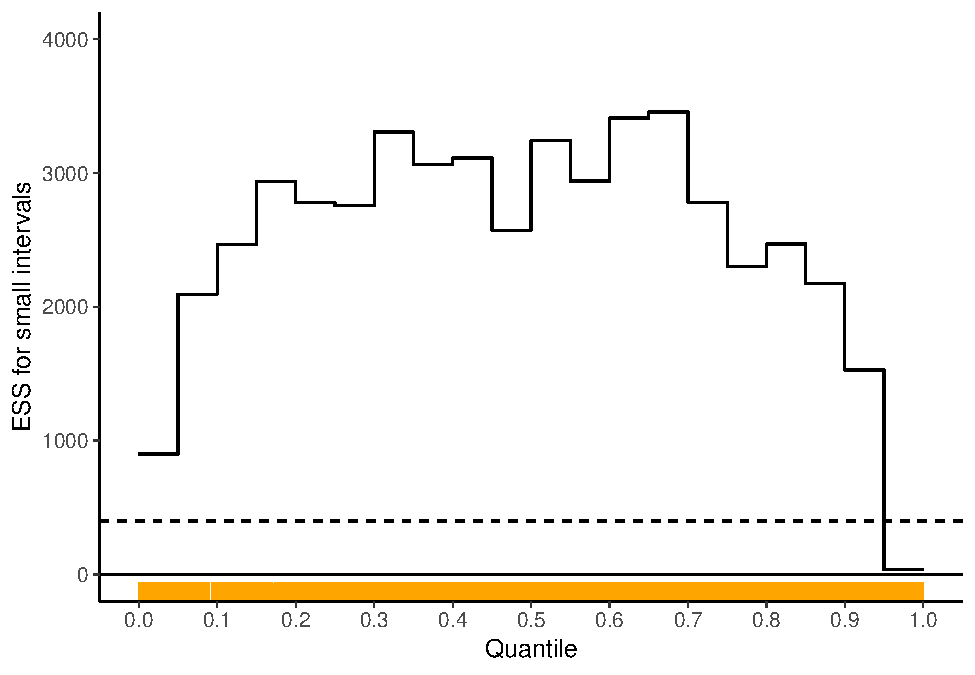
\includegraphics[width=0.98\textwidth]{graphics/local-ess-fit-nom-1.pdf}
  \caption{Local efficiency of small interval probability
    estimates for the Cauchy model with nominal parameterization. Orange
    ticks show iterations that exceeded the maximum treedepth in
    the dynamic HMC algorithm.}
\label{fig:local-ess-fit-nom-1}
\end{minipage}
\hfill
  \begin{minipage}{0.48\textwidth}
  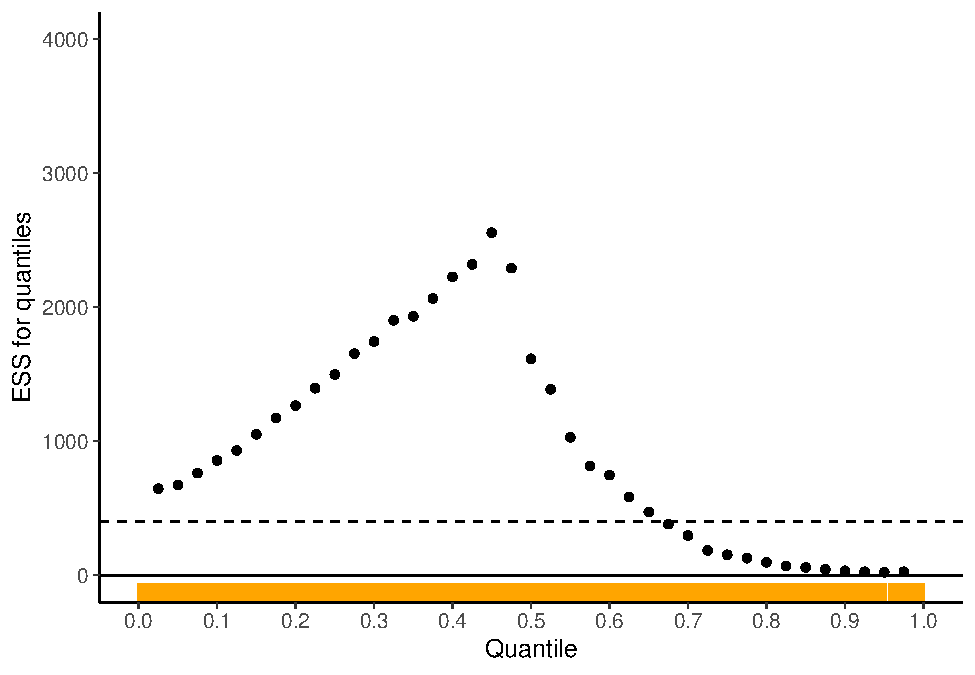
\includegraphics[width=0.98\textwidth]{graphics/quantile-ess-fit-nom-1.pdf}
  \caption{Efficiency of quantile estimates for the Cauchy model with nominal 
  parameterization. Orange ticks show iterations that exceeded the maximum 
  treedepth in the dynamic HMC algorithm.\\~}
  \label{fig:quantile-ess-fit-nom-1}
\end{minipage}
\end{figure}

We may also investigate how the estimated effective sample sizes
change when we use more and more draws (\citet{Brooks+Gelman:1998}
proposed to use similar graph for \(\widehat{R}\)). If the effective
sample size is highly unstable, does not increase proportionally with
more draws, or even decreases, this indicates that simply running
longer chains will likely not solve the convergence issues. In
Figure~\ref{fig:change-ess-fit-nom-1}, we see how unstable both
bulk-ESS and tail-ESS are for this example.
%
Rank plots in Figure~\ref{fig:hist-fit-nom-1} clearly show the
mixing problem between chains. In case of good mixing all rank plots
should be close to uniform. More experiments can be found in Appendix C 
and in the online appendix.

\begin{figure}[tp]
  \centering
  \begin{minipage}{0.48\textwidth}
  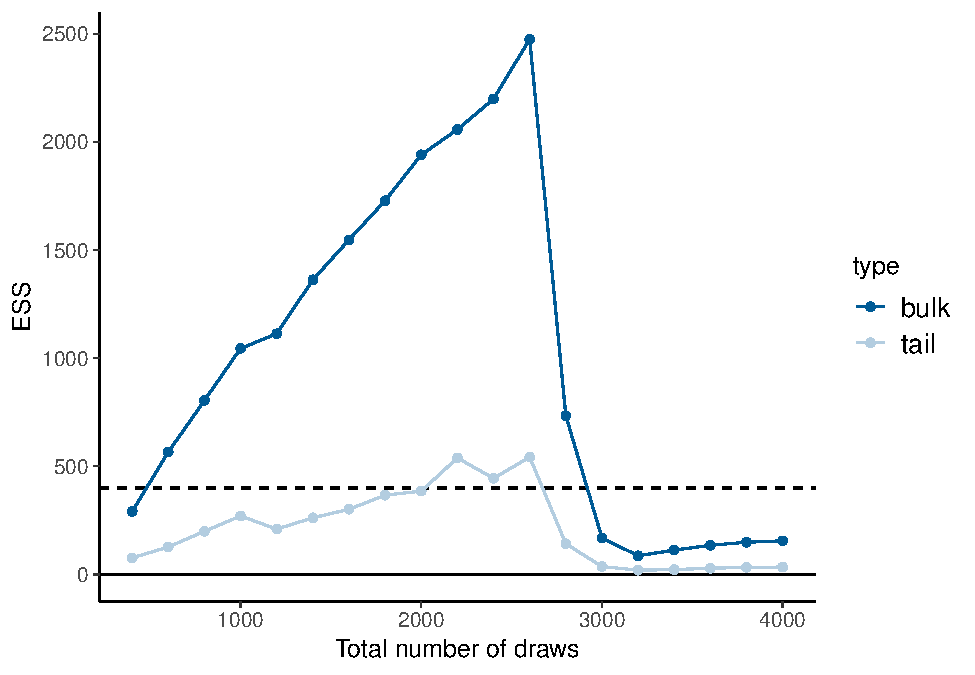
\includegraphics[width=0.98\textwidth]{graphics/change-ess-fit-nom-1.pdf}
  \caption{Estimated effective sample sizes with increasing number of iterations
  for the Cauchy model with nominal parameterization.}
  \label{fig:change-ess-fit-nom-1}
\end{minipage}
\hfill
\begin{minipage}{0.48\textwidth}
  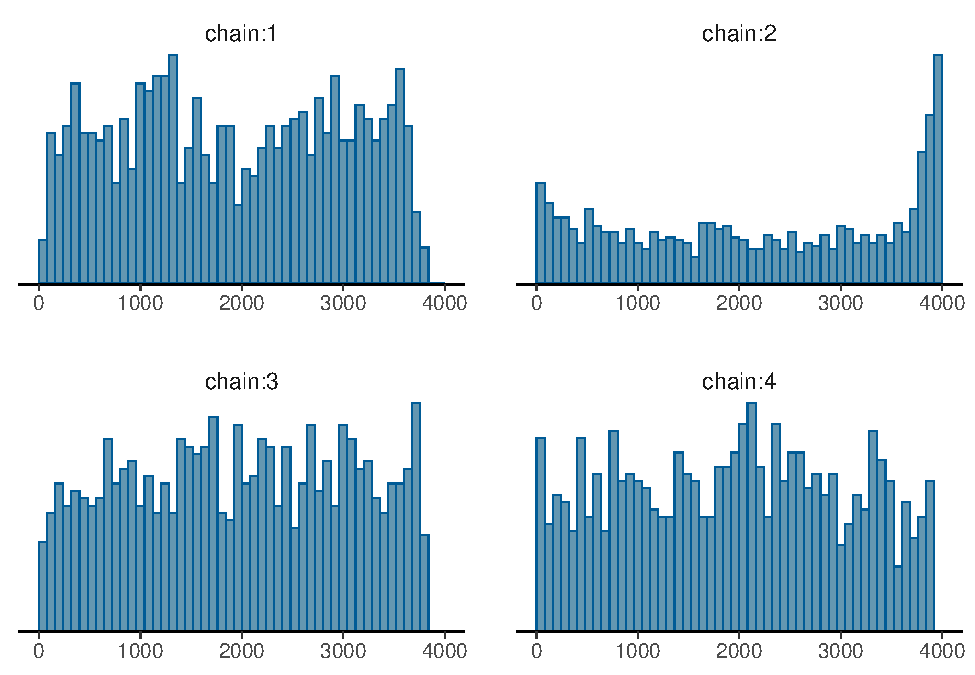
\includegraphics[width=0.98\textwidth]{graphics/hist-fit-nom-1.pdf}
  \caption{Rank plots of posterior draws from four chains for the Cauchy model 
  with nominal parameterization.}
  \label{fig:hist-fit-nom-1}
\end{minipage}
\end{figure}

\hypertarget{alternative-parameterization-of-the-cauchy-distribution}{%
\subsubsection*{Alternative parameterization of the
Cauchy distribution}\label{alternative-parameterization-of-the-cauchy-distribution}}

Next, we examine an alternative parameterization that considers the
Cauchy distribution as a scale mixture of Gaussian distributions
\begin{align}
  a \sim  \N(0,1), \qquad
  b \sim  \Gam (0.5, 0.5), \qquad
  x =  \frac{a}{\sqrt{b}}.
\end{align}
The model has two parameters, and the Cauchy distributed \(x\) can be
computed deterministically from those. In addition to improved sampling 
performance, the example illustrates that focusing on diagnostics matters.
We define two 50-dimensional parameter vectors $a$ and $b$ from which
the 50-dimensional quantity $x$ is computed. There are no warnings and
the sampling is much faster.


For all parameters, the split-\(\widehat{R}\) was less than \(1.01\) and 
ESS was \(>400\), indicating that
sampling worked much better with this alternative parameterization.
The online appendix contains more results using other parameterizations 
of the Cauchy distribution. The vectors \(a\) and \(b\) used
to form the Cauchy distributed \(x\) have stable quantile, mean and
variance values. As \(x\) is Cauchy distributed it has stable
quantiles, but wildly varying mean and variance estimates as the true values
are not finite.
%
We can further analyze potential problems using local efficiency
estimates and rank plots. For this example. we take a detailed look at 
\(x_{40}\), which had the smallest bulk-ESS of 2848.
%
Figures~\ref{fig:local-ess-fit-alt1-1} and
\ref{fig:quantile-ess-alt1-1} show good sampling efficiency for the
small interval probability and quantile estimates.
%
The Rank plots displayed in Figure~\ref{fig:hist-fit-alt1-1} also look quite 
uniform across chains thus indicating convergence.

\begin{figure}[tp]
  \centering
  \begin{minipage}{0.48\textwidth}
  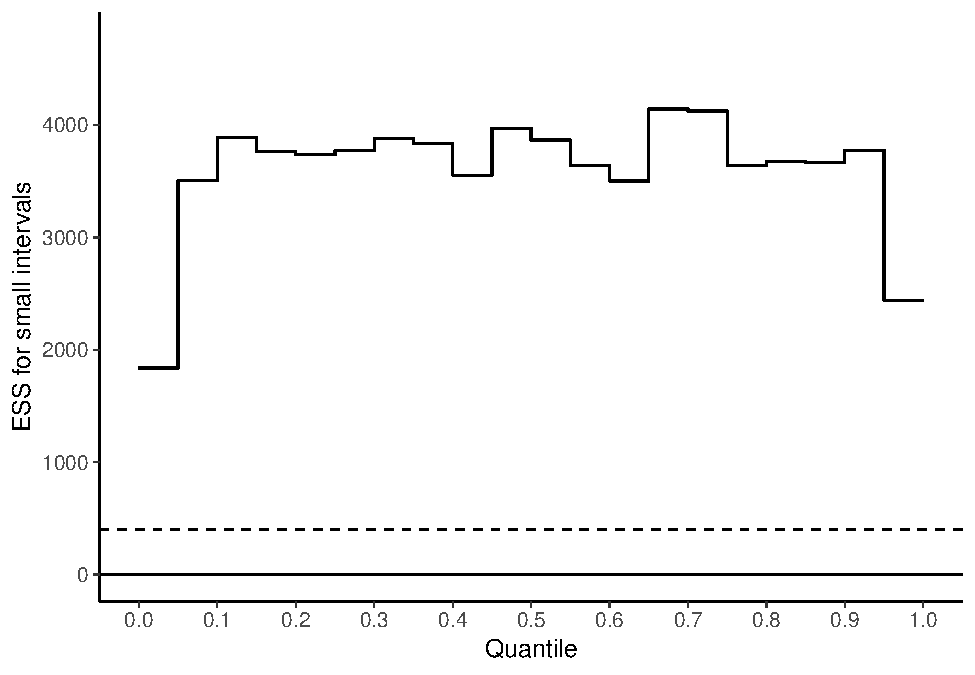
\includegraphics[width=0.98\textwidth]{graphics/local-ess-fit-alt1-1.pdf}
  \caption{Local efficiency of small interval probability estimates for the 
  Cauchy model with alternative parameterization.}
\label{fig:local-ess-fit-alt1-1}
\end{minipage}
\hfill
  \begin{minipage}{0.48\textwidth}
  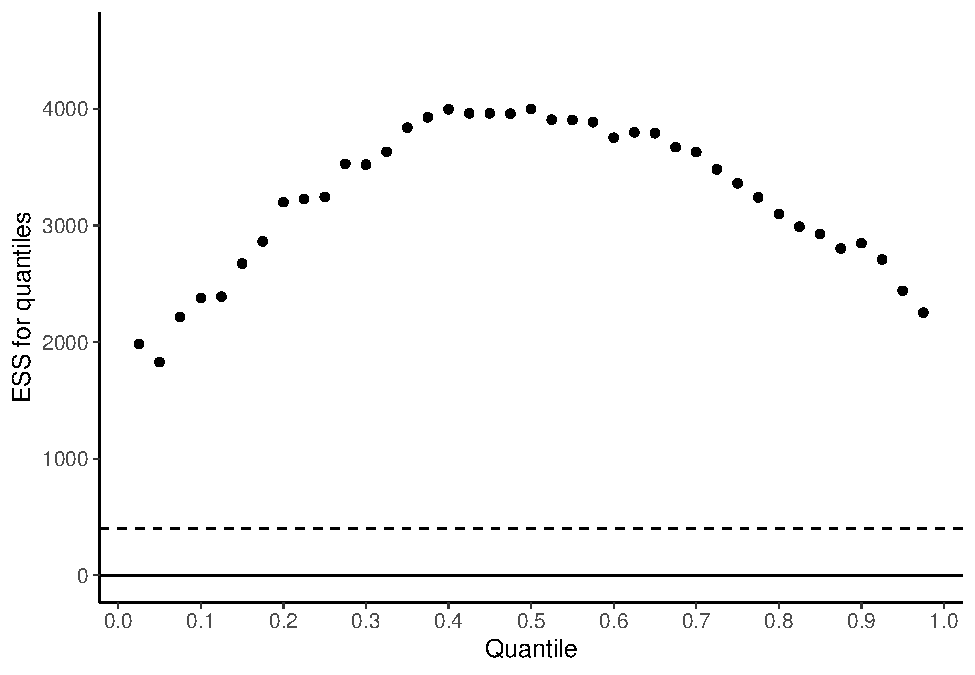
\includegraphics[width=0.98\textwidth]{graphics/quantile-ess-fit-alt1-1.pdf}
  \caption{Efficiency of quantile estimates for the Cauchy model with 
  alternative parameterization.\\~}
  \label{fig:quantile-ess-alt1-1}
\end{minipage}
\end{figure}

\begin{figure}[tp]
  \centering
  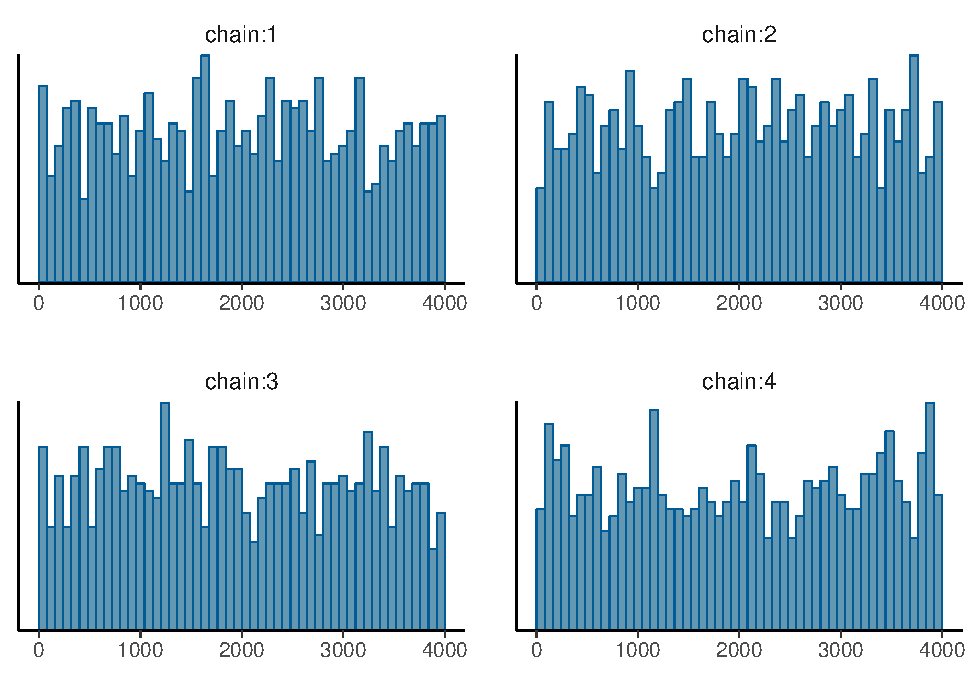
\includegraphics[width=0.47\textwidth]{graphics/hist-fit-alt1-1.pdf}
  \caption{Rank plots of posterior draws from four chains for the Cauchy model with alternative parameterization.}
  \label{fig:hist-fit-alt1-1}
\end{figure}

\hypertarget{half-cauchy-distribution-with-nominal-parameterization}{%
\subsubsection*{Half-Cauchy distribution with nominal
parameterization}\label{half-cauchy-distribution-with-nominal-parameterization}}

Half-Cauchy priors for non-negative parameters are common and, at least in Stan, 
usually specified via the nominal parameterization.
In this example, we set independent half-Cauchy distributions on each element
of the 50 dimensional vector $x$ with positivity constraint
(\texttt{\textless{}lower=0\textgreater{}}). Stan will then
sample automatically in the unconstrained \(\log(x)\) space, which
changes the geometry crucially. As a result, there are no warnings and all
split-\(\widehat{R}<1.01\) and ESS \(>400\) indicate good
performance of the sampler despite using the nominal parameterization of
the Cauchy distribution. More experiments for the half-Cauchy distribution 
can be found in the online appendix.




\hypertarget{eightschools}{%
\subsection{Hierarchical model: Eight schools}\label{eightschools}}

The eight schools problem is a classic example
\citep[see Section 5.5 in][]{BDA3}, which even in its
simplicity illustrates the typical problems in inference for
hierarchical models. We can parameterize this simple model
in at least two ways. The centered parameterization looks as follows:
\begin{align*}
\theta_j &\sim \text{normal}(\mu, \tau) \\
y_j &\sim \text{normal}(\theta_j, \sigma_j)
\end{align*}

In contrast, the non-centered parameterization can be written as:
\begin{align*}
\tilde{\theta}_j &\sim \text{normal}(0, 1) \\
\theta_j &= \mu + \tau \tilde{\theta}_j \\
y_j &\sim \text{normal}(\theta_j, \sigma_j)
\end{align*}

In both parameterizations, $\theta_j$ are the school specific means,
and $\mu$ as well as $\tau$ are the hierarchical mean and standard deviation 
of the school specific means, respectively.

Geometrically, the centered parameterization exhibits a funnel shape
that contracts into a region of strong curvature around small
values of the population standard deviation $\tau$, making it difficult for most
Markov chain methods to adequately explore the full distribution of this
paramater. The online appendix contains more detailed analysis of different 
algorithm variants and results of longer chains.

\hypertarget{a-centered-eight-schools-model}{%
\subsubsection*{A centered eight schools
model}\label{a-centered-eight-schools-model}}

Instead of the default options, we run the centered parameterization
model with more conservative settings of the HMC sample to reduce the
probability of getting divergent transitions. Still, we observe a lot of divergent
transitions, which in itself is already a sufficient indicator of
convergence problems. We may also use the split-\(\widehat{R}\) and ESS
diagnostics to recognize problematic parts of the posterior. The latter
two have the advantage over the divergent transitions diagnostic that they
can be used with all MCMC algorithms not only with HMC.

Bulk-ESS and Tail-ESS for the between school standard deviation $\tau$
are 67 and 82, respectively. Both are much less than 400, indicating we
should investigate that parameter more carefully.
Figures~\ref{fig:local-ess-fit-cp-1} and
\ref{fig:quantile-ess-fit-cp-1} show the sampling efficiency for the
small interval probability and quantile estimates.
The sampler has difficulties in exploring small $\tau$ values. As the
sampling efficiency for small $\tau$ values is practically zero, we
may assume that we miss substantial amount of posterior mass and
get biased estimates. In this case, the severe sampling problems for
small $\tau$ values is reflected in the sampling efficiency for all
quantiles. Red ticks, which show iterations with divergences, have
concentrated to small $\tau$ values, which gives us another indication
of problems in exploring small values.

Figure~\ref{fig:change-ess-fit-cp-1} shows how the estimated effective
sample sizes change when we use more and more draws. Here we do not
see sudden changes, but both bulk-ESS and tail-ESS are consistently low. 
In line with the other findings, rank plots of $\tau$ displayed in
Figure~\ref{fig:hist-fit-cp-1} clearly show problems in the mixing of
the chains.  In particular, the rank plot for the first chain indicates that it was unable to 
explore the lower-end of the posterior range, while the spike in the rank plot 
for chain 2 indicates that it spent too much time stuck in these values.
More experiments can be found in Appendix D and E as well as in the online appendix.


\begin{figure}[tp]
  \centering
  \begin{minipage}{0.48\textwidth}
  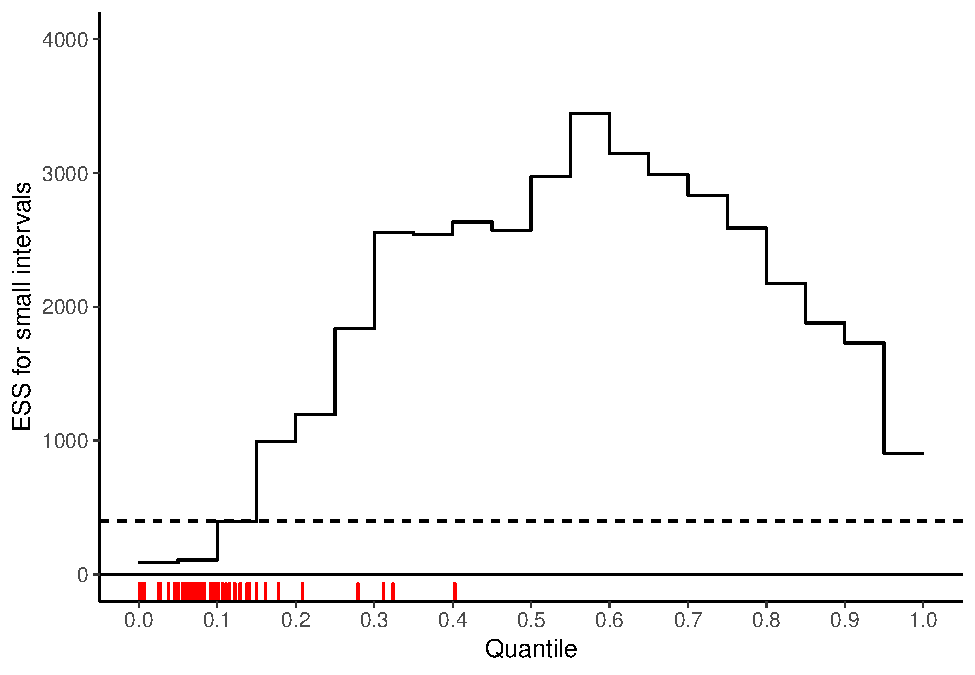
\includegraphics[width=0.98\textwidth]{graphics/local-ess-fit-cp-1.pdf}
  \caption{Local efficiency of small interval probability estimates for the eight  
  schools model with centered parameterization. Red ticks show divergent transitions.}
  \label{fig:local-ess-fit-cp-1}
\end{minipage}
\hfill
  \begin{minipage}{0.48\textwidth}
  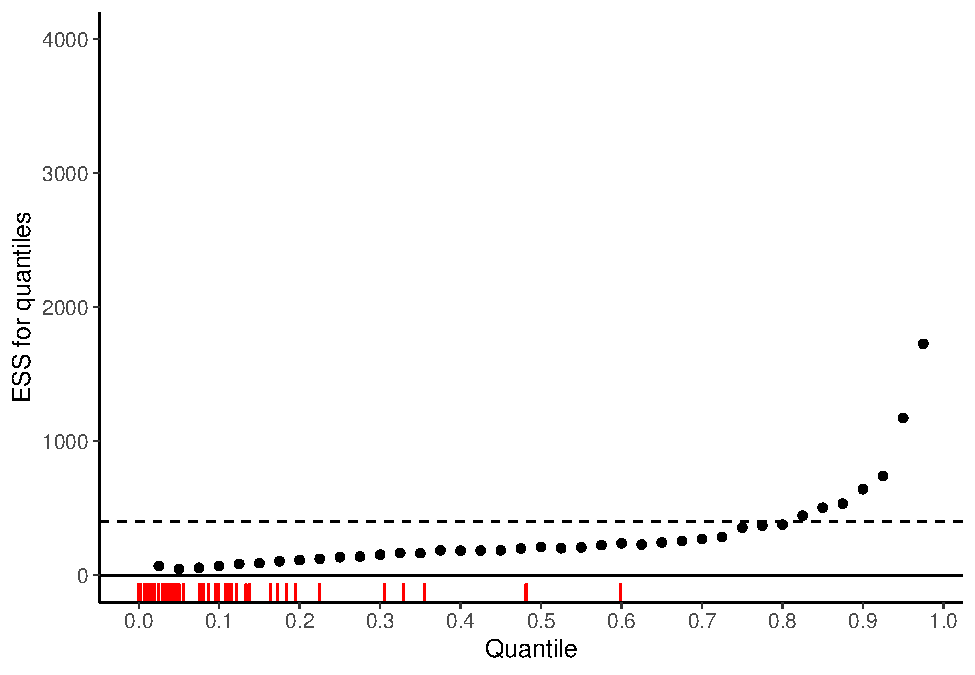
\includegraphics[width=0.98\textwidth]{graphics/quantile-ess-fit-cp-1.pdf}
  \caption{Efficiency of quantile estimates for the eight schools model with 
  centered parameterization. Red ticks show divergent transitions.\\~}
  \label{fig:quantile-ess-fit-cp-1}
 \end{minipage}
\end{figure}


\begin{figure}[tp]
  \centering
  \begin{minipage}{0.48\textwidth}
  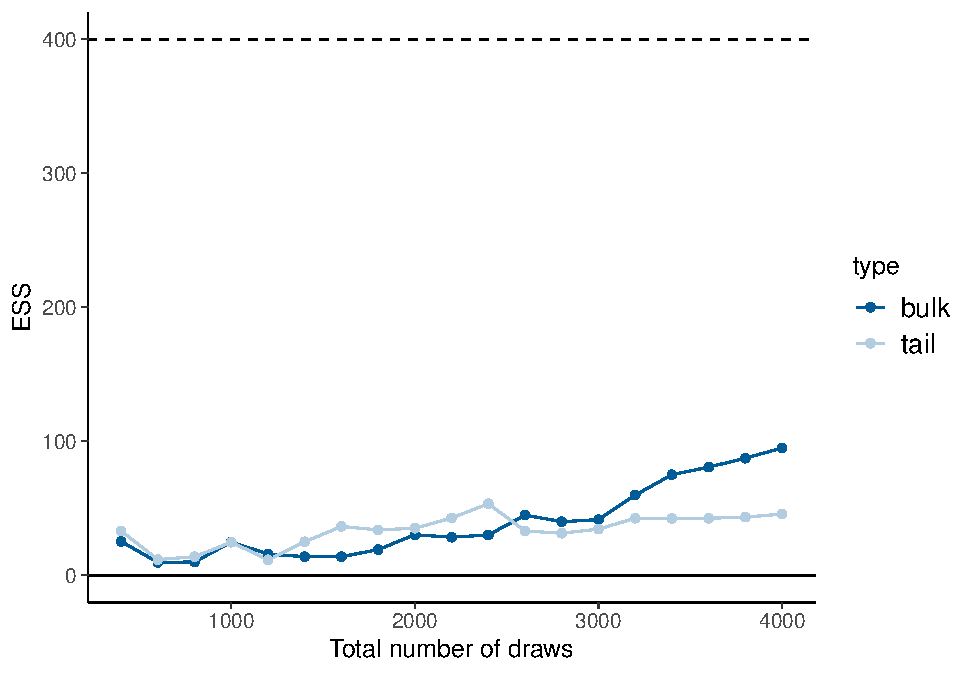
\includegraphics[width=0.98\textwidth]{graphics/change-ess-fit-cp-1.pdf}
  \caption{Estimated effective sample sizes with increasing number of iterations
  for the eight schools model with centered parameterization.}
  \label{fig:change-ess-fit-cp-1}
\end{minipage}
\hfill
  \begin{minipage}{0.48\textwidth}
  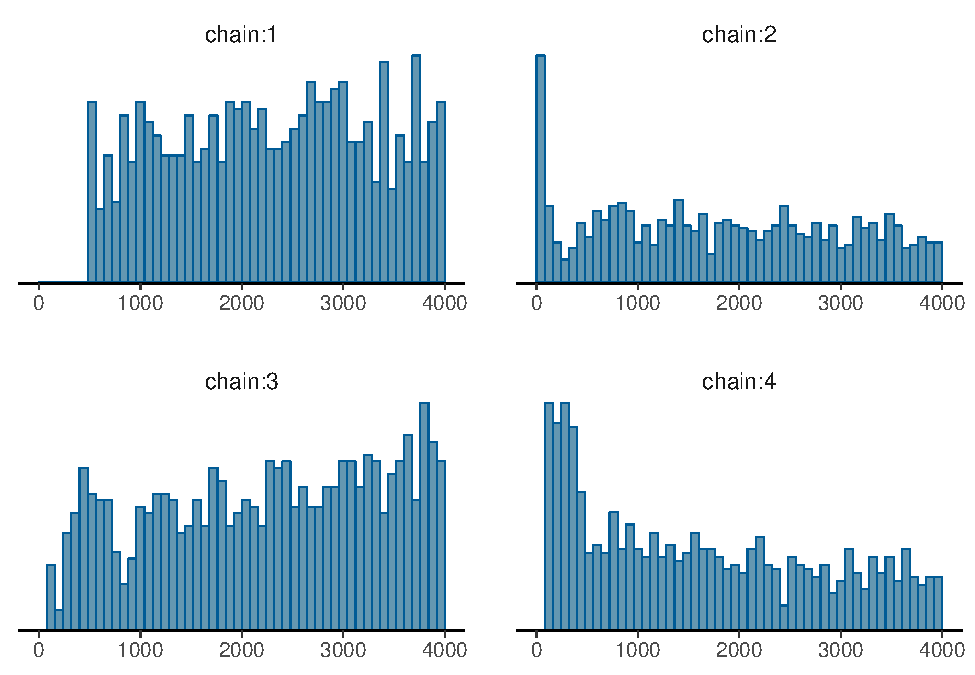
\includegraphics[width=0.98\textwidth]{graphics/hist-fit-cp-1.pdf}
  \caption{Rank plots of posterior draws from four chains for the eight schools 
  model with centered parameterization.}
  \label{fig:hist-fit-cp-1}
\end{minipage}
\end{figure}

\hypertarget{non-centered-eight-schools-model}{%
\subsubsection*{Non-centered eight schools
model}\label{non-centered-eight-schools-model}}

For hierarchical models, the corresponding non-centered
parameterization often works better. For reasons of comparability, we use the 
same conservative sampler setting as for the centered parameterization model. 
For the non-centered parameterization, we do not observe divergences or 
other warnings.
All split-\(\widehat{R}<1.01\) and ESS \(>400\) indicate a much
better efficiency of the non-centered parameterization.
Figures~\ref{fig:local-ess-fit-ncp2-1} and
\ref{fig:quantile-ess-fit-ncp2-1} show the efficiency of small interval
probability estimates and the efficiency of quantile estimates for
$\tau$.
Small $\tau$ values are still more difficult to explore, but the relative 
efficiency is good. The rank plots of $\tau$ Figure~\ref{fig:hist-fit-ncp2-1} 
show no substantial differences between chains.


\begin{figure}[tp]
  \begin{minipage}{0.48\textwidth}
  \centering
  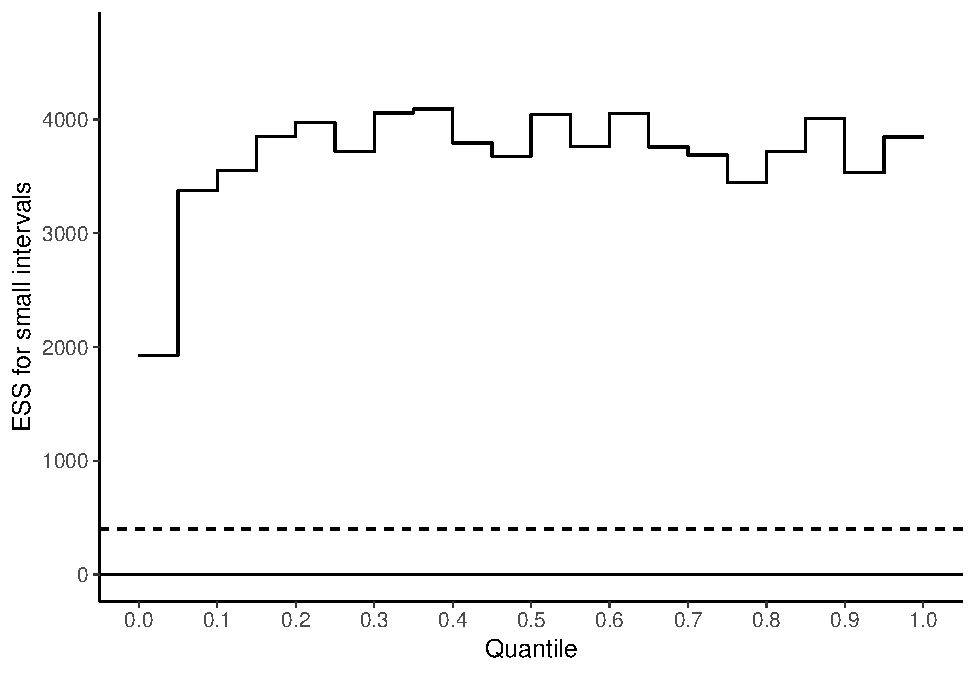
\includegraphics[width=0.98\textwidth]{graphics/local-ess-fit-ncp2-1.pdf}
  \caption{Local efficiency of small interval probability estimates for the  
  eight schools model with the non-centered parameterization.}
  \label{fig:local-ess-fit-ncp2-1}
\end{minipage}
\hfill
  \begin{minipage}{0.48\textwidth}
  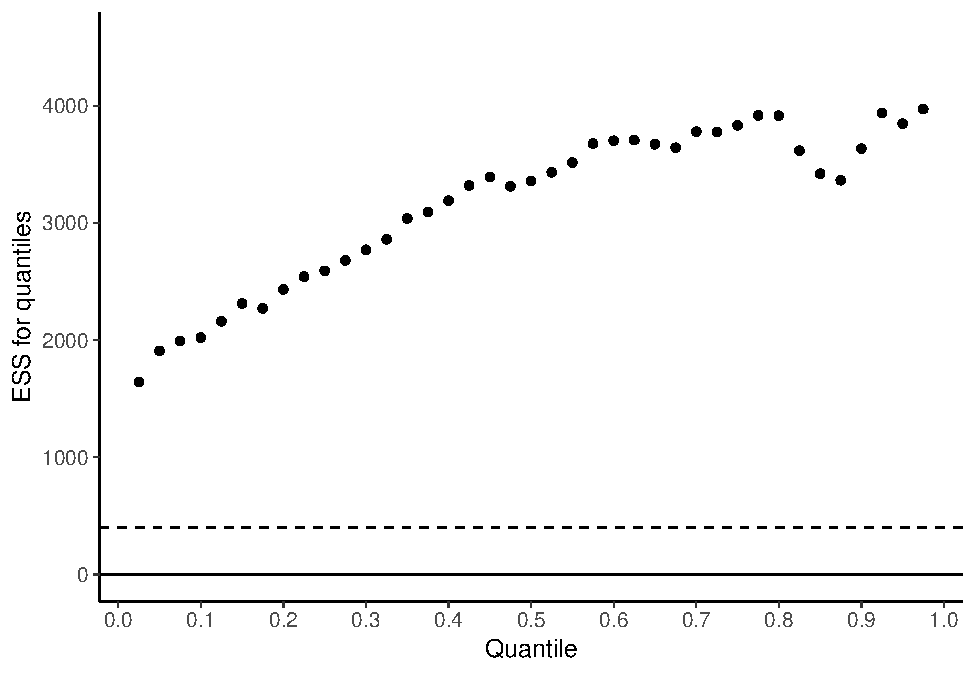
\includegraphics[width=0.98\textwidth]{graphics/quantile-ess-fit-ncp2-1.pdf}
  \caption{Efficiency of quantile estimates for the eight schools model with 
  the non-centered parameterization.}
  \label{fig:quantile-ess-fit-ncp2-1}
\end{minipage}
\end{figure}

\begin{figure}[tp]
  \centering
  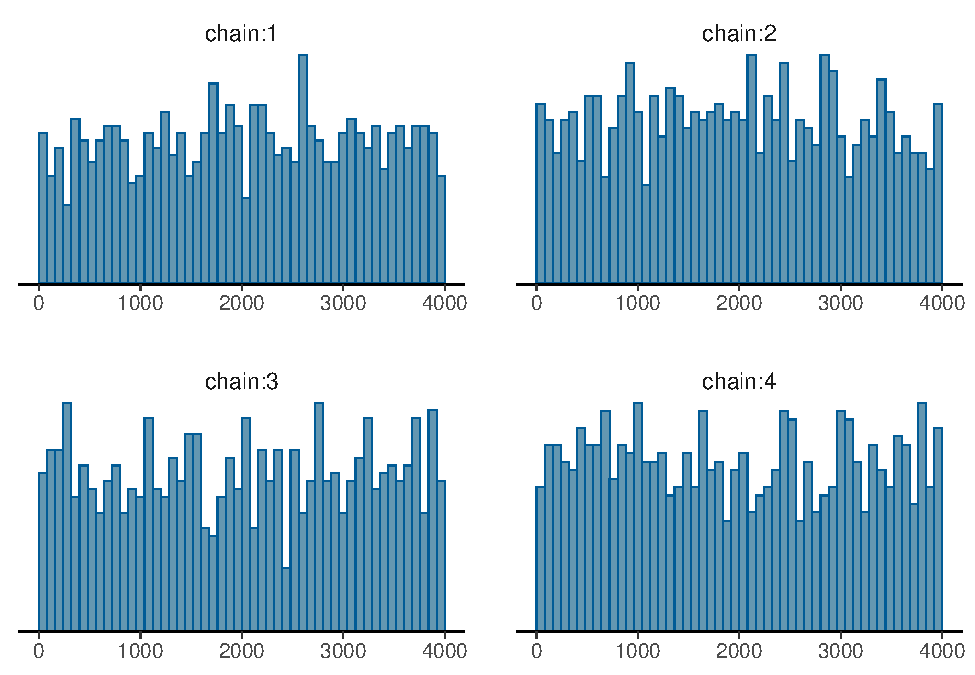
\includegraphics[width=0.47\textwidth]{graphics/hist-fit-ncp2-1.pdf}
  \caption{Rank plots of posterior draws from four chains for 8 schools model with non-centered parameterization.}
  \label{fig:hist-fit-ncp2-1}
\end{figure}


\hypertarget{refs}{}

\bibliography{rhat}

\newpage
\hypertarget{ESS}{%
\subsection*{Appendix A: Computing the effective sample size}\label{ESS}}

If the \(N\) simulation draws within each chain were truly independent,
the between-chain variance \(B\) would be an unbiased estimate of the
posterior variance, \(\mbox{var}(\theta | y)\), and we would have a
total of \(S = MN\) independent simulations from the \(M\) chains. In
general, however, the simulations of \(\theta\) within each chain will
be autocorrelated, and thus \(B\) will be larger than
\(\mbox{var}(\theta | y)\), in expectation.

One way to define effective sample size for correlated simulation draws
is to consider the statistical efficiency of the average of the
simulations \(\bar{\theta}^{(..)}\) as an estimate of the posterior mean
\(\mbox{E}(\theta | y)\). This also generalizes to posterior
expectations of functionals of parameters \(\mbox{E}\left(g(\theta) | y\right)\).
Section \ref{convergence-diagnostics-for-quantiles} deals with 
estimating the effective sample size of
quantiles, which cannot be presented as expectations. For simplification,
in this section we consider the effective sample size for the posterior
mean.

The effective sample size of a chain is defined in terms of the
autocorrelations within the chain at different lags. The autocorrelation
\(\rho_t\) at lag \(t \geq 0\) for a chain with joint probability
function \(p(\theta)\) with mean \(\mu\) and standard deviation \(\sigma\) is
defined to be

\begin{equation}
\rho_t = \frac{1}{\sigma^2} \, \int_{\Theta} (\theta^{(n)} - \mu)
(\theta^{(n+t)} - \mu) \, p(\theta) \, d \theta.
\end{equation}

This is just the correlation between the two chains offset by \(t\)
positions. Because we know \(\theta^{(n)}\) and \(\theta^{(n+t)}\) have
the same marginal distribution in an MCMC setting, multiplying the two
difference terms and reducing yields

\begin{equation}
\rho_t = \frac{1}{\sigma^2} \, \int_{\Theta} \theta^{(n)} \, \theta^{(n+t)}
\, p(\theta) \, d \theta.
\end{equation}

The effective sample size of one chain generated by a process with
autocorrelations \(\rho_t\) is defined by

\begin{equation}
N_{\rm eff} \ = \
\frac{N}{\sum_{t = -\infty}^{\infty} \rho_t} \ = \
\frac{N}{1 + 2 \sum_{t = 1}^{\infty} \rho_t}.
\end{equation}

The effective sample size \(N_{\rm eff}\) can be larger than \(N\) in case
of antithetic Markov chains, which have negative autocorrelations on odd
lags. The dynamic Hamiltonian Monte Carlo algorithms used in Stan
\citep{Hoffman+Gelman:2014, betancourt2017conceptual} can produce
\(N_{\rm eff}>N\) for parameters with a close to Gaussian posterior (in
the unconstrained space) and low dependence on the other parameters.

In practice, the probability function in question cannot be tractably
integrated and thus neither autocorrelation nor the effective sample
size can be directly calculated. Instead, these quantities must be estimated from
the samples themselves. The rest of this section describes an
autocorrelation and split-\(\widehat{R}\) based effective sample size
estimator, based on multiple split chains. For simplicity, each chain
will be assumed to be of the same length \(N\).

Computations of autocorrelations for all lags simultaneously can be done
via the fast Fourier transform algorithm \citep[FFT; see][]{Geyer:2011}. 
The autocorrelation estimates \(\hat{\rho}_{t,m}\)
at lag \(t\) from multiple chains \(m \in (1,\ldots,M)\) are combined
with the within-chain variance estimate \(W\) and the multi-chain
variance estimate \(\widehat{\mbox{var}}^{+}\) introduced above to
compute the combined autocorrelation at lag \(t\) as,

\begin{equation}
\hat{\rho}_t
= 1 - \frac{\displaystyle W - \textstyle \frac{1}{M}\sum_{m=1}^M 
\hat{\rho}_{t,j}}{\widehat{\mbox{var}}^{+}}. \label{rhohat}
\end{equation}

If the chains have not converged, the variance estimator
\(\widehat{\mbox{var}}^{+}\) will overestimate the true marginal
variance which leads to an overestimation of the autocorrelation and an
underestimation of the effective sample size.

Because of noise in the correlation estimates \(\hat{\rho}_t\) increases
as \(t\) increases, typically the truncated sum of \(\hat{\rho}_t\) is
used. Negative autocorrelations can happen only on odd lags and by
summing over pairs starting from lag \(t=0\), the paired autocorrelation
is guaranteed to be positive, monotone and convex modulo estimator noise
\citep{Geyer:1992, Geyer:2011}. The effective sample size of combined
chains is then defined as,

\begin{equation}
S_{\rm eff} = \frac{N \, M}{\hat{\tau}},
\end{equation} where \begin{equation}
\hat{\tau} = 1 + 2 \sum_{t=1}^{2k+1} \hat{\rho}_t = 
-1 + 2 \sum_{t'=0}^{k} \hat{P}_{t'},
\end{equation}

and \(\hat{P}_{t'}=\hat{\rho}_{2t'}+\hat{\rho}_{2t'+1}\). The initial
positive sequence estimator is obtained by choosing the largest \(k\)
such that \(\hat{P}_{t'}>0\) for all \(t' = 1,\ldots,k\). The initial
monotone sequence estimator is obtained by further reducing
\(\hat{P}_{t'}\) to the minimum of the preceding values so that the
estimated sequence becomes monotone.

The effective sample size \(S_{\rm eff}\) described here is different
from similar formulas in the literature in that we use multiple chains
and between-chain variance in the computation, which typically gives us
more conservative claims (lower values of \(S_{\rm eff}\)) compared to
single chain estimates, especially when mixing of the chains is poor. If
the chains are not mixing at all (e.g., if the posterior is multimodal and
the chains are stuck in different modes), then our \(S_{\rm eff}\) is
close to the number of distinct modes that are found (i.e., very small).



\hypertarget{AppendixD}{%
\subsection*{Appendix B: Normal distributions with additional trend,
shift or scaling}\label{AppendixD}}
\addcontentsline{toc}{subsection}{Appendix B: Normal distributions with
additional trend, shift or scaling}

Here we demonstrate the behavior of non-split-\(\widehat{R}\),
split-\(\widehat{R}\), and bulk-ESS to detect various simulated cases
presenting non-convergence behavior. We generate four varying length
chains of iid normally distributed values, and then modify them to
simulate three convergence problems:
\begin{itemize}
\tightlist
\item All chains have the same trend and a similar marginal
  distribution. This can happen in case of slow mixing and all chains
  initialized near each other far from the typical set.
\item One of the chains has a different mean. This can happen in case
  of slow mixing, weak identifiability of one or several parameters, or
  multimodality.
\item One of the chains having a lower marginal variance. This can
  happen in case of slow mixing, multimodality, or one of the chains
  having different mixing efficiency.
\end{itemize}


\hypertarget{adding-the-same-trend-to-all-chains}{%
\paragraph{All chains have the same trend.}\label{adding-the-same-trend-to-all-chains}}
First we draw all the chains are from the same $\N(0, 1)$ distribution plus
a linear trend. Figure~\ref{fig:rhat-same-trend-1}
shows that if we don't split chains, \(\widehat{R}\) misses the trends
if all chains still have a similar marginal distribution.
%
Figure~\ref{fig:zsrhat-same-trend-1} shows that split-\(\widehat{R}\)
detects the trend, even if the marginals of the chains are similar. If
we use a threshold of \(1.01\), we can detect trends which account for
2\% or more of the total marginal variance. If we use a threshold of
\(1.1\), we detect trends which account for 30\% or more of the total
marginal variance.
\begin{figure}[tp]
  \centering
  \begin{minipage}{0.48\textwidth}
  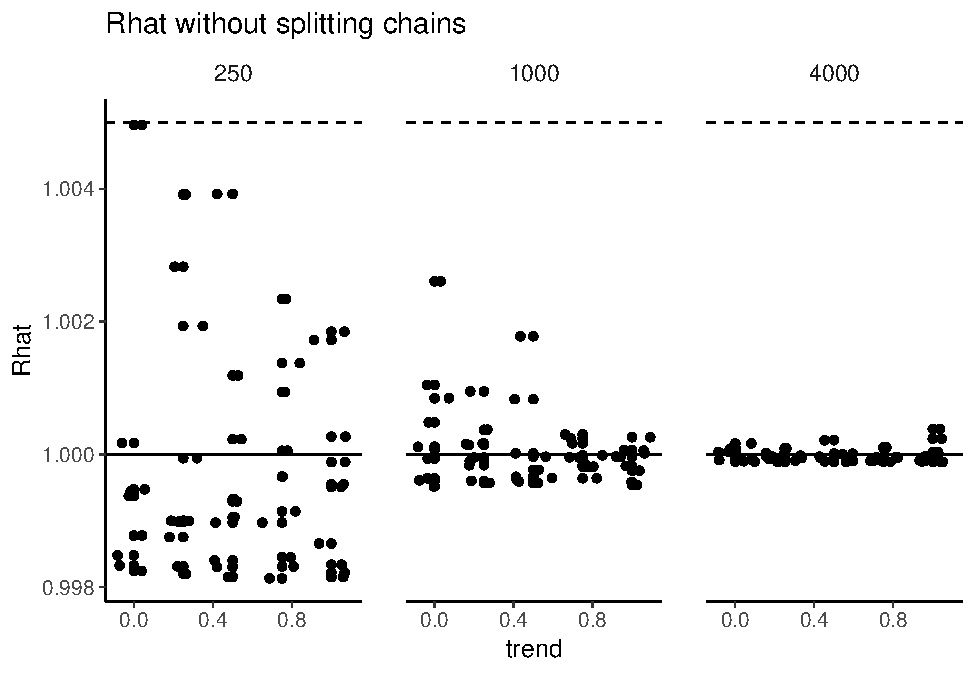
\includegraphics[width=0.98\textwidth]{graphics/rhat-same-trend-1.pdf}
  \caption{\(\widehat{R}\) without splitting for varying chain lengths
    for chains which have the same trend and a similar marginal
    distribution.}
  \label{fig:rhat-same-trend-1}
\end{minipage}
\hfill
  \begin{minipage}{0.48\textwidth}
  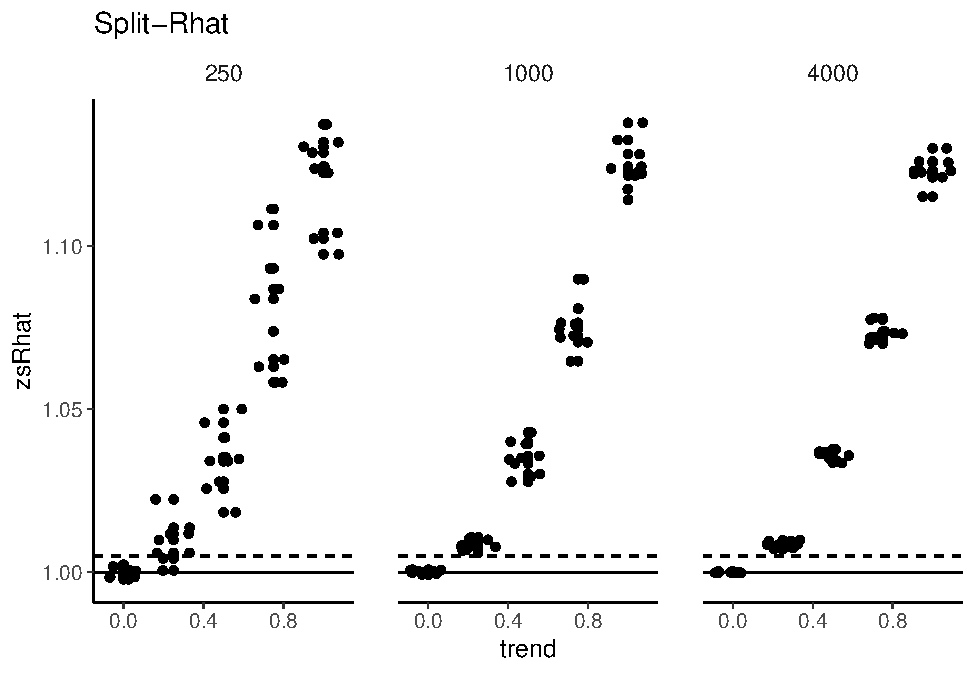
\includegraphics[width=0.98\textwidth]{graphics/zsrhat-same-trend-1.pdf}
  \caption{Split-\(\widehat{R}\) for varying chain lengths
    for chains which have the same trend and a similar marginal
    distribution.}
  \label{fig:zsrhat-same-trend-1}
\end{minipage}
\end{figure}

The effective sample size is based on split-\(\widehat{R}\) and
within-chain autocorrelation. Figure~\ref{fig:zsreff-same-trend-1}
shows the relative Bulk-ESS divided by \(S\) for easier
comparison between different values of \(S\).
%
We see that split-\(\widehat{R}\) is more sensitive to trends for
small sample sizes, but ESS becomes more sensitive for larger samples
sizes (as autocorrelations can be estimated more accurately).
\begin{figure}[tp]
  \centering
  \begin{minipage}{0.48\textwidth}
  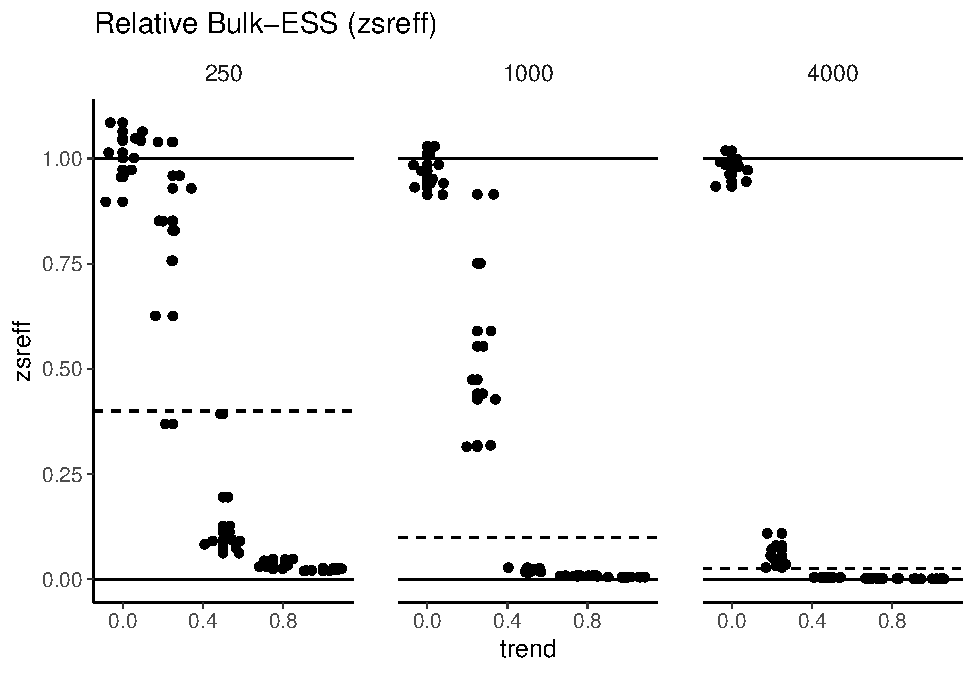
\includegraphics[width=0.98\textwidth]{graphics/zsreff-same-trend-1.pdf}
  \caption{Relative Bulk-ESS for varying chain lengths for chains which have
    the same trend and a similar marginal distribution. The dashed
    lines indicate the threshold \(S_{\rm eff} > 400\) at which we
    would consider the effective sample size to be sufficient.}
  \label{fig:zsreff-same-trend-1}
\end{minipage}
\hfill
  \begin{minipage}{0.48\textwidth}
  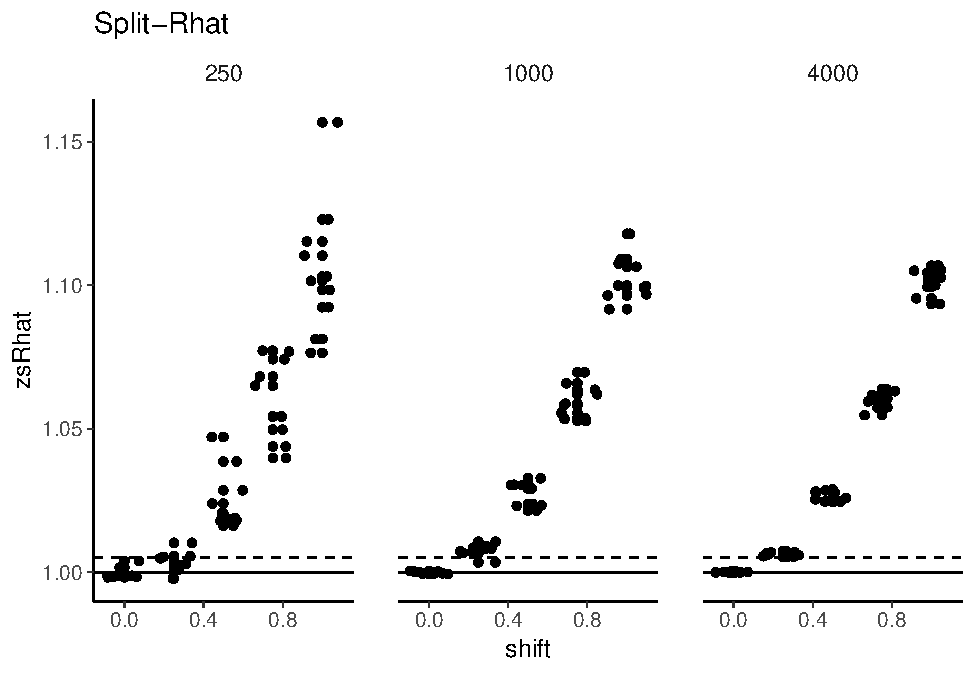
\includegraphics[width=0.98\textwidth]{graphics/zsrhat-shifted-chain-1.pdf}
  \caption{Split-\(\widehat{R}\) for varying chain lengths
    for chains with one sampled with a different mean than the others.\\~\\~}
  \label{fig:zsrhat-shifted-chain-1}
\end{minipage}
\end{figure}

\hypertarget{shifting-one-chain}{%
\paragraph{Shifting one chain.}\label{shifting-one-chain}}
Second  we draw all the chains are from the same $\N(0, 1)$ distribution,
except one that is sampled with non-zero
mean. Figure~\ref{fig:zsrhat-shifted-chain-1} shows that if we use a
threshold of \(1.01\), split-\(\widehat{R}\) can detect shifts with a
magnitude of one third or more of the marginal standard deviation. If
we use a threshold of \(1.1\), split-\(\widehat{R}\) detects shifts
with a magnitude equal to or larger than the marginal standard
deviation.
%
Figure~\ref{fig:zsreff-shifted-chain-1} shows the the relative
Bulk-ESS for the same case. The effective
sample size is not as sensitive as split-\(\widehat{R}\), but a shift
with a magnitude of half the marginal standard deviation or more will
lead to very low relative efficiency when the total number of draws
increases.
\begin{figure}[tp]
  \centering
  \begin{minipage}{0.48\textwidth}
  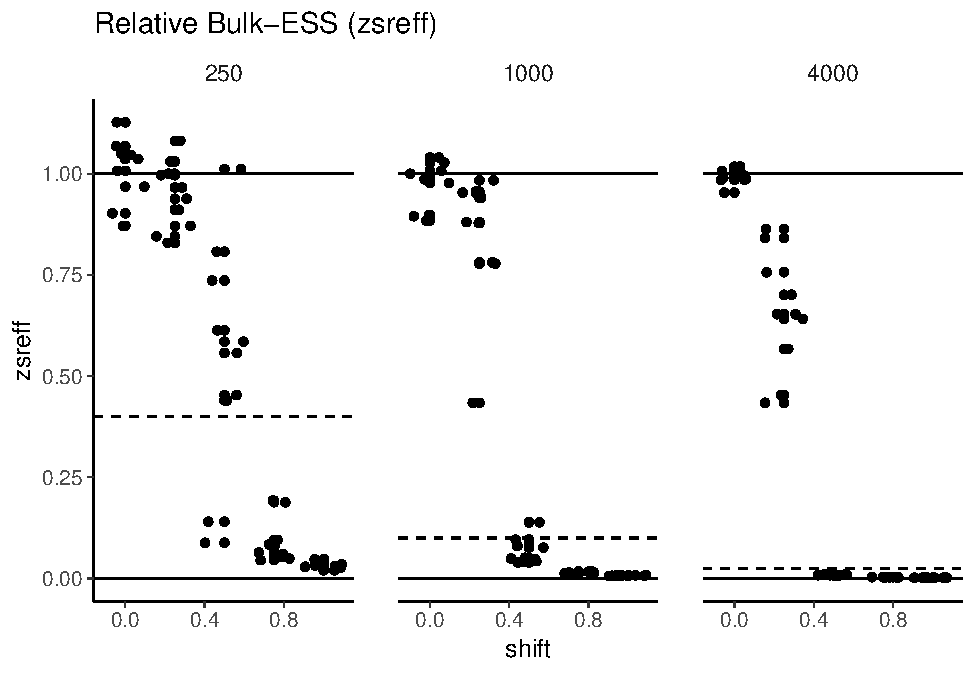
\includegraphics[width=0.98\textwidth]{graphics/zsreff-shifted-chain-1.pdf}
  \caption{Relative Bulk-ESS for varying chain lengths for chains with one
    sampled with a different mean than the others. The dashed lines
    indicate the threshold \(S_{\rm eff} > 400\) at which we would
    consider the effective sample size to be sufficient.}
  \label{fig:zsreff-shifted-chain-1}
\end{minipage}
\hfill
  \begin{minipage}{0.48\textwidth}
  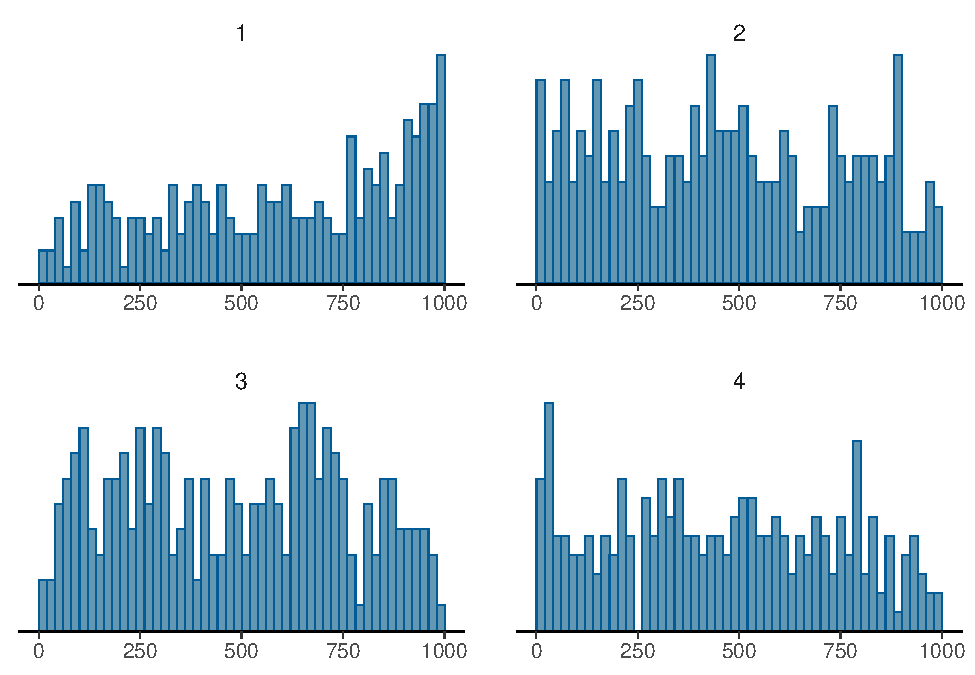
\includegraphics[width=0.98\textwidth]{graphics/hist-shifted-chain-1.pdf}
  \caption{Rank plots of posterior draws from four chains with one
    sampled with a different mean than the others.\\~\\}
  \label{fig:hist-shifted-chain-1}
\end{minipage}
\end{figure}
Rank plots are practical way to visualize differences between
chains. Figure~\ref{fig:hist-shifted-chain-1} shows rank plots for the
case of 4 chains, 250 draws per chain, and one chain sampled with mean
0.5 instead of 0. In this case split-\(\widehat{R} = 1.05\), but the
rank plots clearly show that the first chain behaves differently.

\hypertarget{scaling-one-chain}{%
\paragraph{Scaling one chain.}\label{scaling-one-chain}}
For our third simulation, all the chains are from the same $\N(0, 1)$ distribution,
except one of the chains is sampled with variance less than 1.
Figure~\ref{fig:zsrhat-scaled-chain-1} shows that
split-\(\widehat{R}\) is not able to detect scale differences between
chains.
%
Figure~\ref{fig:zfsrhat-scaled-chain-1} shows that
folded-split-\(\widehat{R}\) which focuses on scales detects scale
differences. With a threshold of \(1.01\),
folded-split-\(\widehat{R}\) detects a chain with scale less than
\(3/4\) of the standard deviation of the others. With a threshold of
\(1.1\), folded-split-\(\widehat{R}\) detects a chain with standard
deviation less than \(1/4\) of the standard deviation of the others.
\begin{figure}[tp]
  \centering
  \begin{minipage}{0.48\textwidth}
  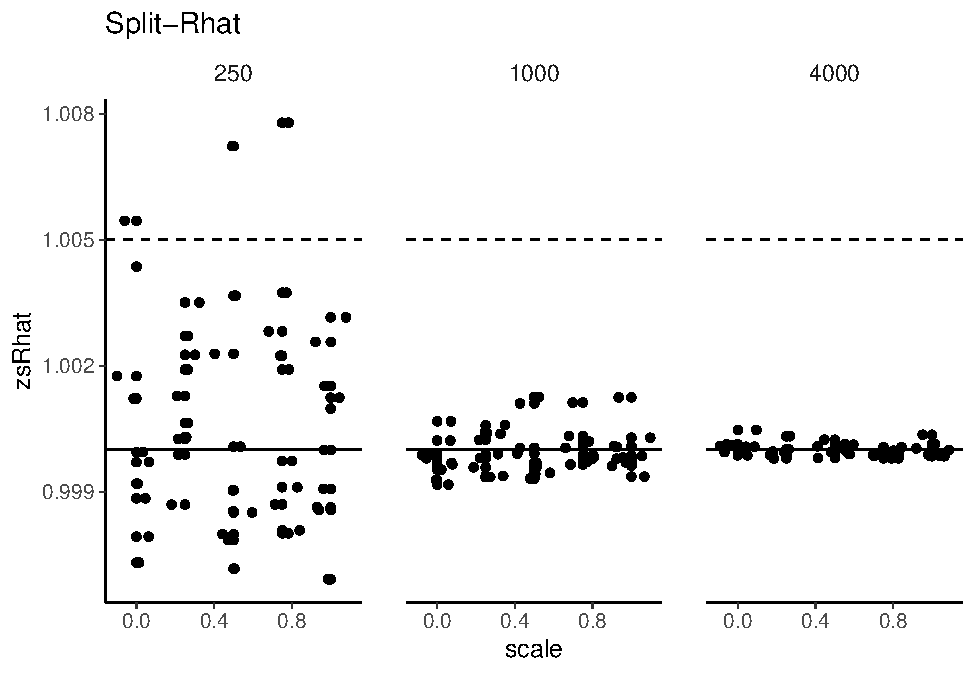
\includegraphics[width=0.98\textwidth]{graphics/zsrhat-scaled-chain-1.pdf}
  \caption{Split-\(\widehat{R}\) for varying chain lengths
    for chains with one sampled with a different variance than the others.}
  \label{fig:zsrhat-scaled-chain-1}
\end{minipage}
\hfill
  \begin{minipage}{0.48\textwidth}
  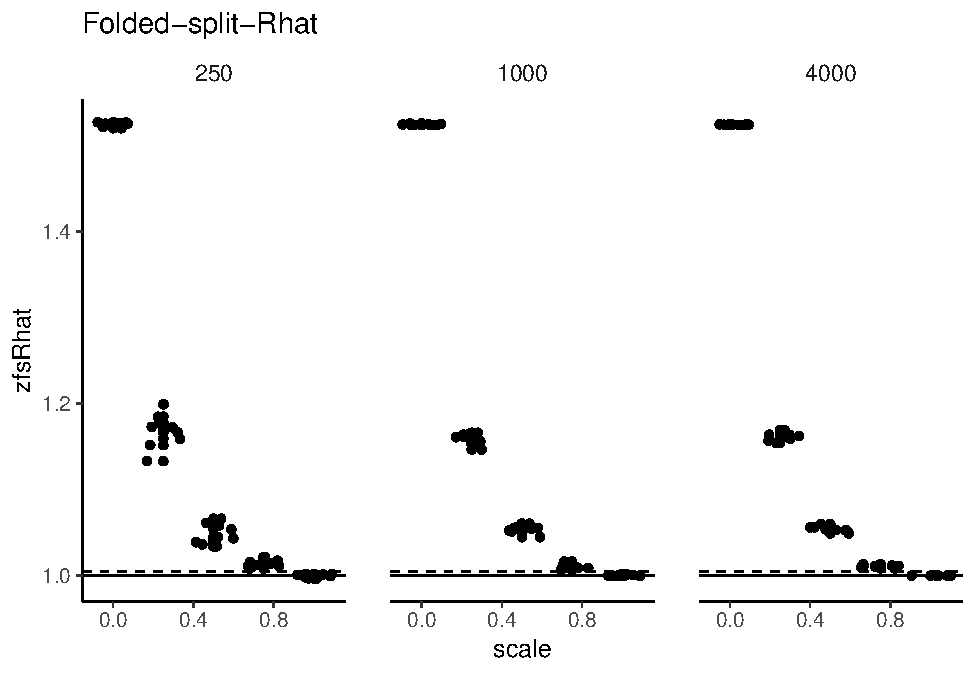
\includegraphics[width=0.98\textwidth]{graphics/zfsrhat-scaled-chain-1.pdf}
  \caption{Folded-split-\(\widehat{R}\) for varying chain lengths
    for chains with one sampled with a different variance than the others.}
  \label{fig:zfsrhat-scaled-chain-1}
\end{minipage}
\end{figure}

Figure~\ref{fig:zsreff-scaled-chain-1} shows the the relative Bulk-ESS
for the same case. The bulk effective sample
size of the mean does not see a problem as it focuses on location
differences between chains.
\begin{figure}[tp]
  \centering
  \begin{minipage}{0.48\textwidth}
  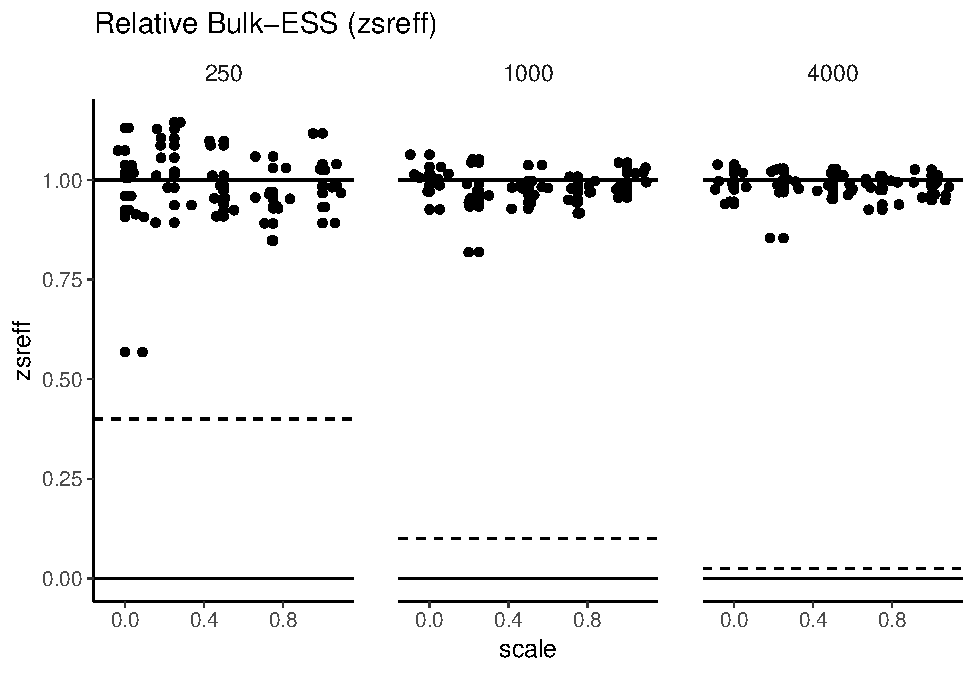
\includegraphics[width=0.98\textwidth]{graphics/zsreff-scaled-chain-1.pdf}
  \caption{Relative Bulk-ESS for varying chain lengths for chains with
    one sampled with a different variance than the others.}
  \label{fig:zsreff-scaled-chain-1}
\end{minipage}
\hfill
  \begin{minipage}{0.48\textwidth}
  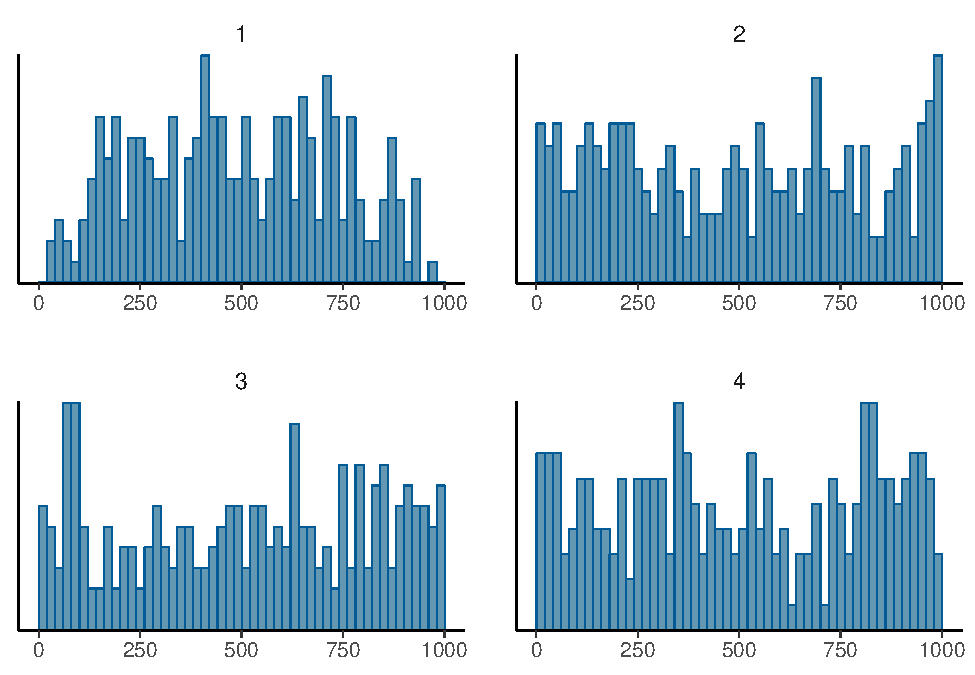
\includegraphics[width=0.98\textwidth]{graphics/hist-scaled-chain-1.pdf}
  \caption{Rank plots of posterior draws from four chains with
    one sampled with a different variance than the others.}
  \label{fig:hist-scaled-chain-1}
\end{minipage}
\end{figure}
Figure~\ref{fig:hist-scaled-chain-1} shows rank plots for the case of
4 chains, 250 draws per chain, and one chain sampled with standard
deviation 0.75 instead of 1. Although
folded-split-\(\widehat{R} = 1.06\), the rank plots clearly show that
the first chain behaves differently.

\hypertarget{AppendixC}{%
\subsection*{Appendix C: More experiments with the Cauchy distribution}\label{AppendixE}}
\addcontentsline{toc}{subsection}{Appendix C: More experiments with the Cauchy distribution}

Here we provide some additional results for the the nominal Cauchy
model presented in the main text. Instead of the default options we
increase \texttt{max\_treedepth} to \(20\), which improves the
exploration in long tails. The online appendix has additional results
for the default option case and for longer chains.


Figure~\ref{fig:trace-fit-nom-td20-1} shows that trace plots for the first
parameter look wild with occasional large values, and it is difficult
to interpret possible convergence.
\begin{figure}[tp]
  \centering
  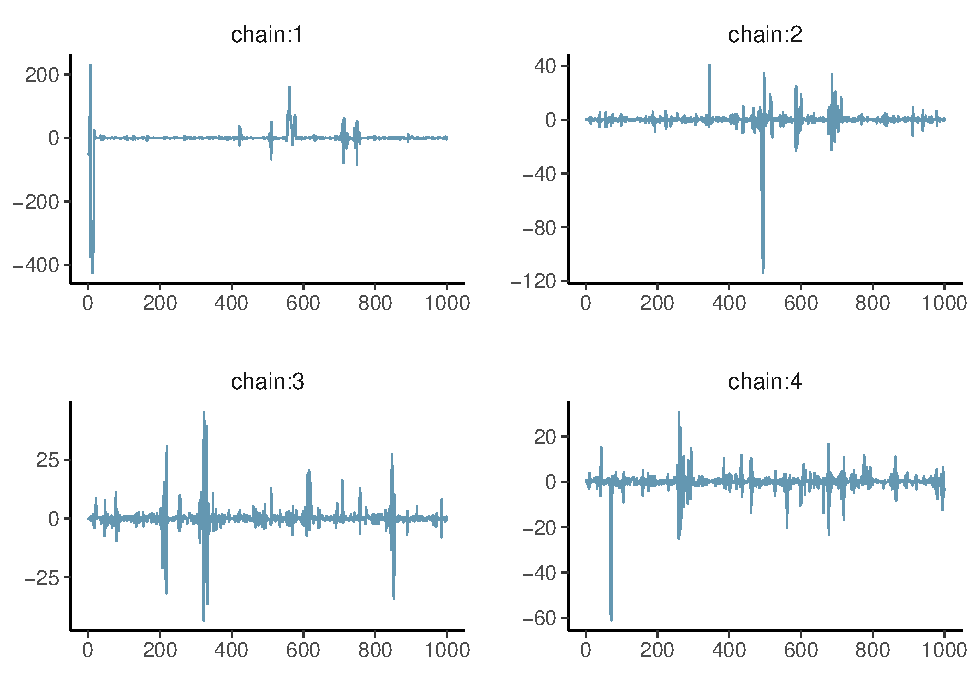
\includegraphics[width=0.47\textwidth]{graphics/trace-fit-nom-td20-1.pdf}
  \caption{Trace plots of four chains for Cauchy model with nominal parameterization and \texttt{max\_treedepth}=20.\\~}
  \label{fig:trace-fit-nom-td20-1}
\end{figure}
%
Figure~\ref{fig:rhat-fit-nom-td20-1} shows classic split-\(\widehat{R}\) ,
rank normalized split-\(\widehat{R}\), and rank normalized
folded-split-\(\widehat{R}\) for all 50 parameters. Classic split-\(\widehat{R}\), which is
not well-defined in this case, has much higher variability than rank
normalized split-\(\widehat{R}\).  Rank normalized
folded-split-\(\widehat{R}\) has higher values than rank normalized
split-\(\widehat{R}\) indicating slow mixing especially in tails.
% 
\begin{figure}[tp]
  \centering
  \begin{minipage}{0.48\textwidth}
  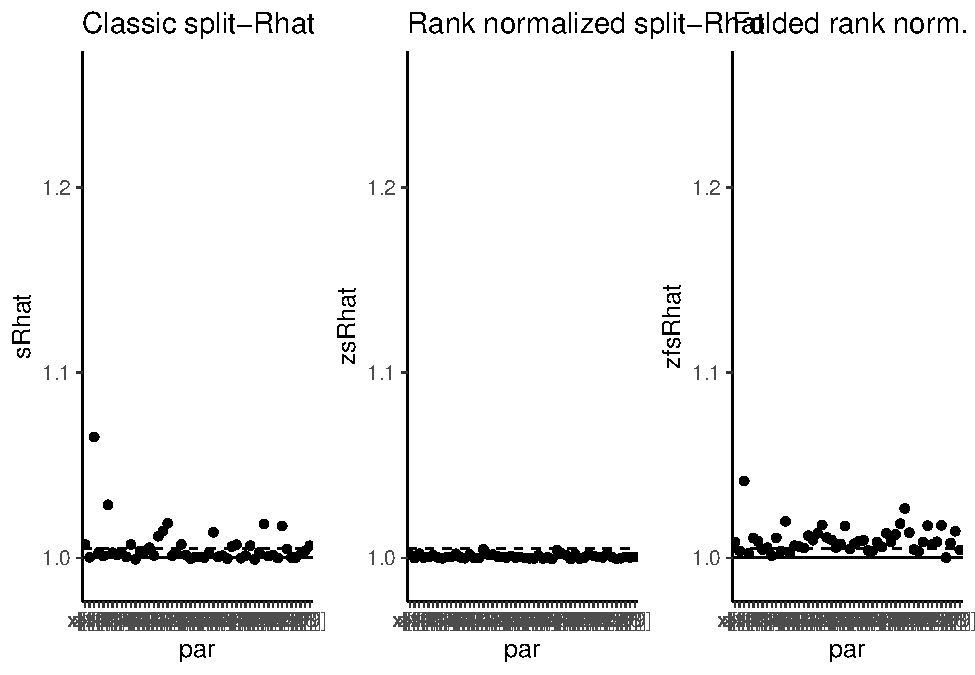
\includegraphics[width=0.98\textwidth]{graphics/rhat-fit-nom-td20-1.pdf}
  \caption{Classic split-\(\widehat{R}\), rank normalized
    split-\(\widehat{R}\), and rank normalized
    folded-split-\(\widehat{R}\) for Cauchy model with nominal
    parameterization and \texttt{max\_treedepth}=20.}
  \label{fig:rhat-fit-nom-td20-1}
\end{minipage}
\hfill
  \begin{minipage}{0.48\textwidth}
  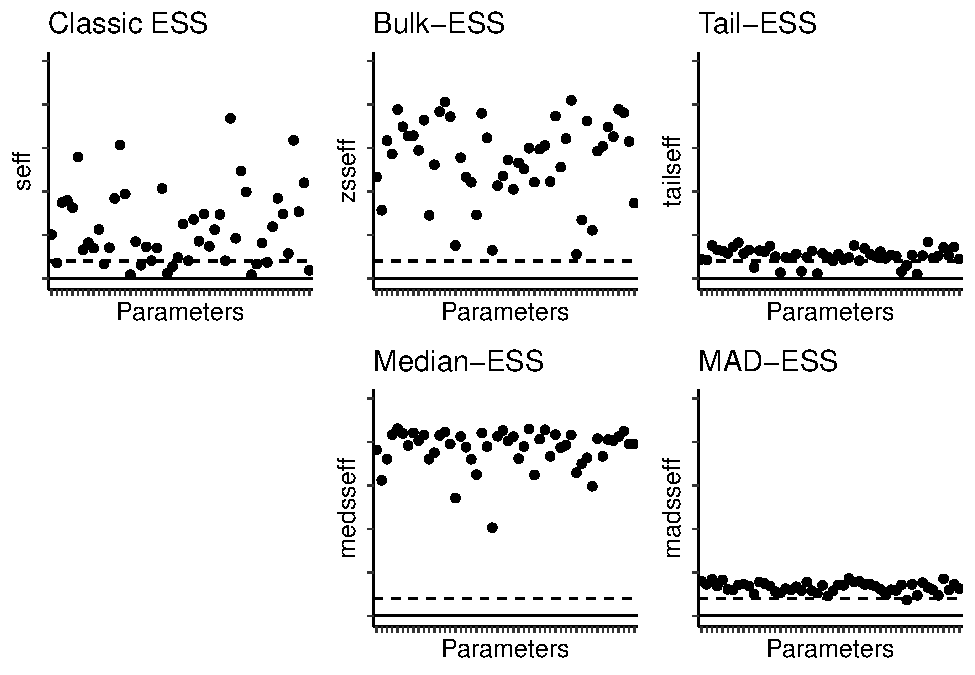
\includegraphics[width=0.98\textwidth]{graphics/ess-fit-nom-td20-1.pdf}
  \caption{Classic ESS, Bulk-ESS, Tail-ESS, Median-ESS and MAD-ESS for
    Cauchy model with nominal parameterization \texttt{max\_treedepth}=20.}
  \label{fig:ess-fit-nom-td20-1}
\end{minipage}
\end{figure}
Figure~\ref{fig:rhat-fit-nom-td20-1} shows different effective sample
size estimates for all 50 parameters. Classic ESS, which is not well
defined in this case, has very high variability. Bulk ESS is much more
stable, and indicates that we can get reliable estimates for the
location of the posterior (except for mean). Median ESS is even more
stable with relatively high values, indicating that we can estimate
median of the distribution reliably. Tail-ESS has low values,
indicating still too slow mixing in tails for reliable tail quantile
estimates. MAD ESS values are just above our recommend threshold,
indicating practically useful MAD estimates, too. The online appendix
has additional results with longer chains, showing that all other ESS
values except classic ESS (which is not well defined) keep improving
with more iterations. It is however recommended to use more efficient
parameterization especially if the tail quantiles are quantities of
interest.


\hypertarget{a-centered-eight-schools-model-1}{%
\subsection*{Appendix D: A centered eight schools model with very long chains and
thinning}\label{a-centered-eight-schools-model-1}}
\addcontentsline{toc}{subsection}{Appendix D: A centered eight schools model}


Here we demonstrate a limitation of split-\(\widehat{R}\) and ESS as a
convergence diagnostics in case where the chains eventually converge
to a common wrong stationary distribution.

When autocorrelation time is high, it has been common to thin the
chains by saving only a small portion of the draws. This will throw
away useful information also for convergence diagnostics. We run the
eight schools model with centered parameterization with $4\times 10^5$
iterations per chain. We remove the first half as warm-up and thin by
200, ending up with 4000 iterations as with the default settings.

We observe several divergent transitions and the estimated Bayesian
fraction of missing information is also low, which still indicate
convergence problems and potentially biased estimates.

Figures \ref{fig:local-ess-fit-cp4-tau-1},
\ref{fig:quantile-ess-fit-cp4-tau-1}, and
\ref{fig:change-ess-fit-cp4-tau-1} show the efficiency of small
probability interval estimates, efficiency of quantile estimates, and
change of Bulk-SS and Tail-ESS with increasing number of iterations.
Unfortunately the thinning makes split-\(\widehat{R}\) and ESS
estimates to miss the problems. The posterior mean is still biased,
being more than 3 sigmas away from the estimate obtained using
non-centered parameterization. In this case all four chains fail
similarly in exploring the narrowest part of the funnel and all
chains seem to ``converge'' to a wrong stationary distribution.
\begin{figure}[tp]
  \centering
  \begin{minipage}{0.48\textwidth}
  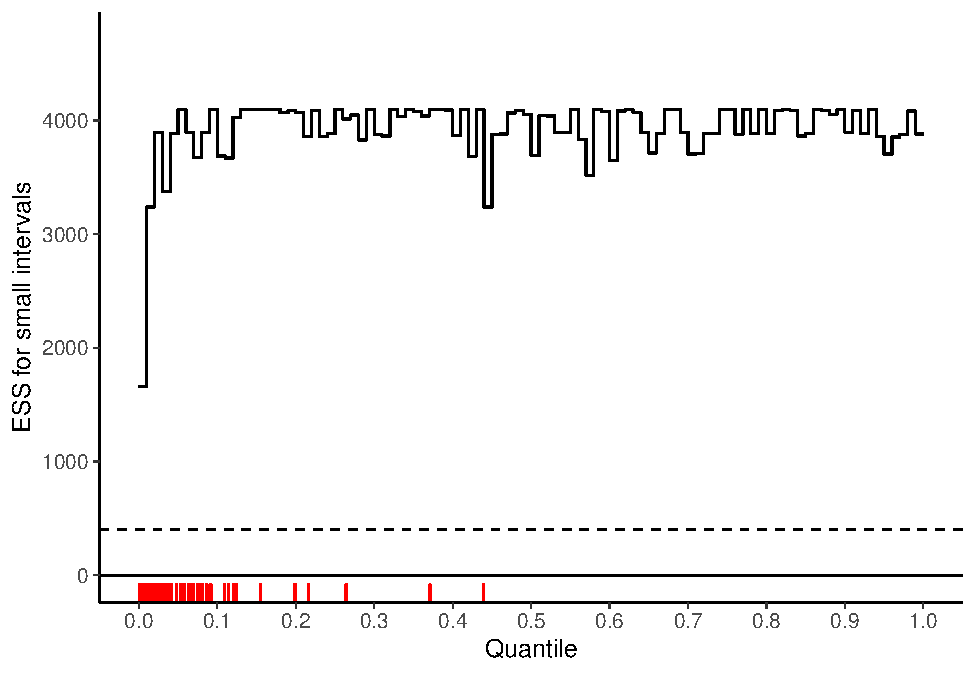
\includegraphics[width=0.98\textwidth]{graphics/local-ess-fit-cp4-tau-1.pdf}
  \caption{The local efficiency of small interval probability estimates for 8 schools model with centered parameterization, very long chains, and thinning.}
  \label{fig:local-ess-fit-cp4-tau-1}
\end{minipage}
\hfill
  \begin{minipage}{0.48\textwidth}
  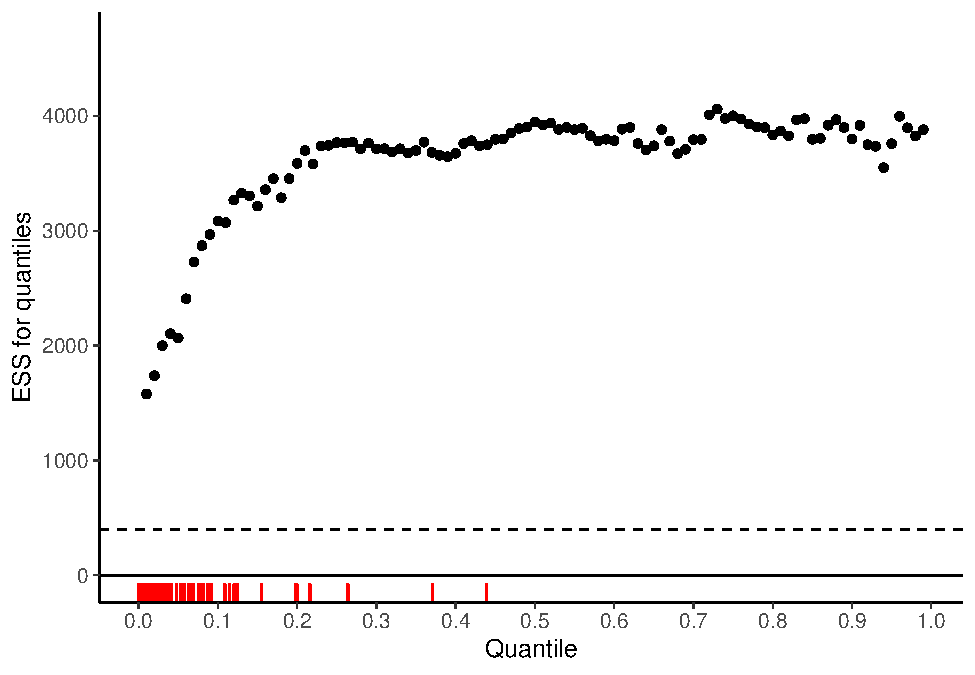
\includegraphics[width=0.98\textwidth]{graphics/quantile-ess-fit-cp4-tau-1.pdf}
  \caption{The efficiency of quantile estimates for 8 schools model with centered parameterization, very long chains, and thinning.}
  \label{fig:quantile-ess-fit-cp4-tau-1}
\end{minipage}
\end{figure}
\begin{figure}[tp]
  \centering
  \begin{minipage}{0.48\textwidth}
  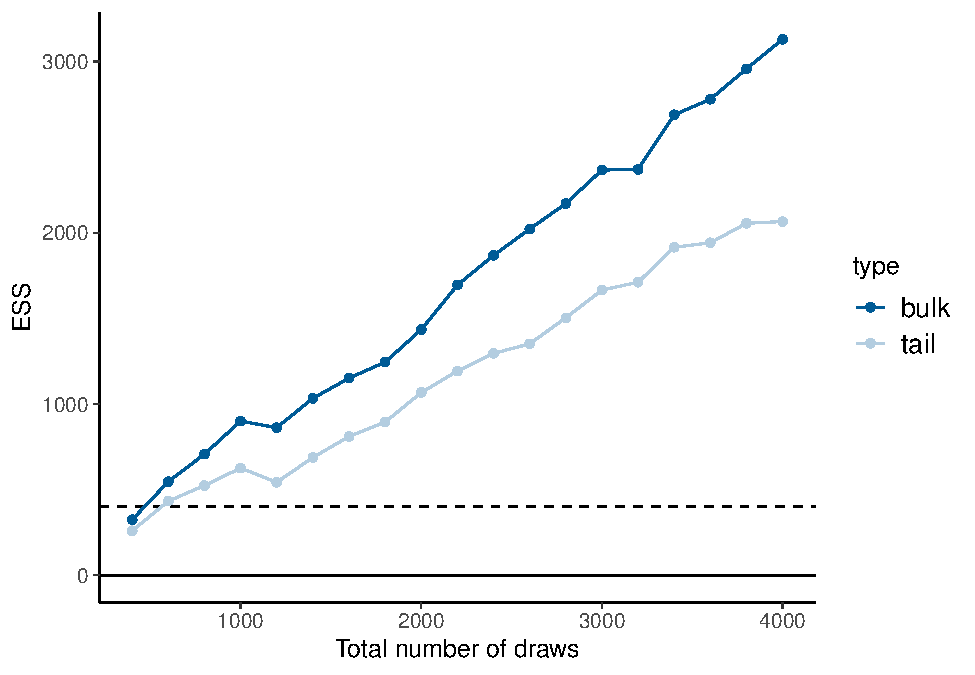
\includegraphics[width=0.98\textwidth]{graphics/change-ess-fit-cp4-tau-1.pdf}
  \caption{The estimated effective sample sizes with increasing number of iterations for 8 schools model with centered parameterization, very long chains, and thinning.}
  \label{fig:change-ess-fit-cp4-tau-1}
\end{minipage}
\hfill
  \begin{minipage}{0.48\textwidth}
  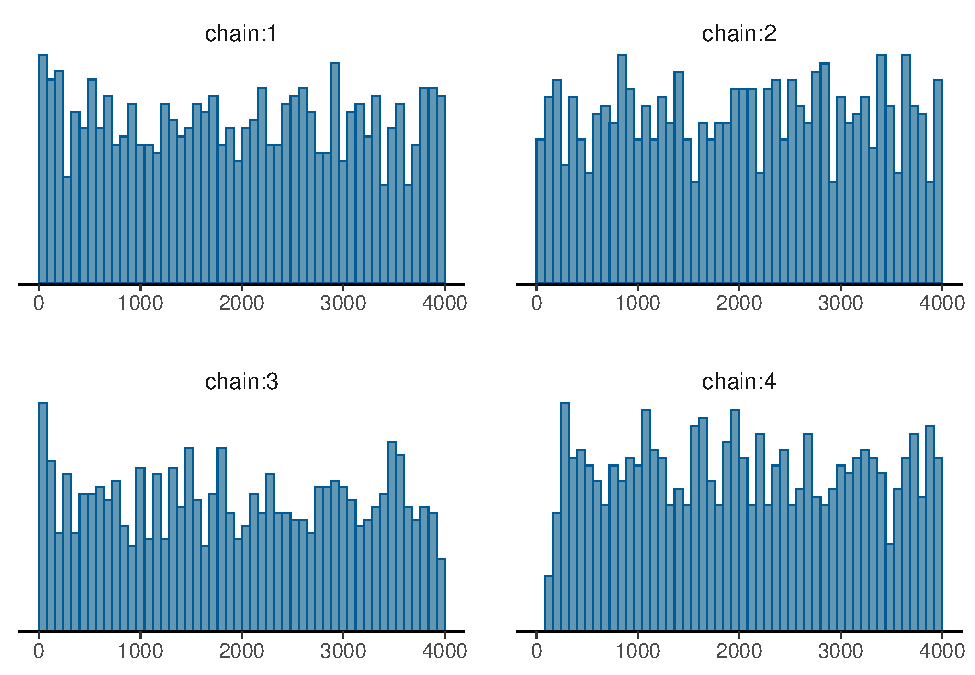
\includegraphics[width=0.98\textwidth]{graphics/hist-fit-cp4-tau-1.pdf}
  \caption{Rank plots of posterior draws from four chains for 8
    schools model with centered parameterization, very long chains, and
    thinning.}
  \label{fig:hist-fit-cp4-tau-1}
\end{minipage}
\end{figure}
However, the rank plots shown in Figure~\ref{fig:hist-fit-cp4-tau-1}
are still able to show the problem.


\hypertarget{eight-schools-with-jags}{%
\subsection*{Appendix E: A centered eight schools model fit using a Gibbs sampler}\label{eight-schools-with-jags}}
\addcontentsline{toc}{subsection}{Appendix E: Eight Schools with Jags}

So far, we have run all models in Stan, but here we demonstrate that
these diagnostics are  also usefult for samplers other than 
Hamiltonian Monte Carlo.  We fit the eight schools models also with
 Jags \citep{plummer2003jags}, which uses a dialect of the BUGS
language \citep{lunn2009bugs} to specify models. Jags uses a clever
mix of Gibbs and Metropolis-Hastings sampling. This kind of sampling
does not usually scale well to high-dimensional posteriors with strongly
dependent parameters \citep[see, e.g.][]{Hoffman+Gelman:2014}, but it can work fine for relatively simple models such as in this case study.


First, we sample 1000 iterations for each of the 4 chains for easy
comparison with the corresponding Stan results. Examining the
diagnostics for $\tau$, Split-\(\widehat{R}=1.08\), Bulk-ESS$=59$, and
Tail-ESS$=53$. 1000 iterations is clearly not enough. The online
appendix shows also the usual visual diagnostics for 1000 iterations
run, but here we next report the results with 10\,000 iterations.
Examining the diagnostics for $\tau$, now Split-\(\widehat{R}=1.01\),
Bulk-ESS$=677$, and Tail-ESS$=1027$, which are all good.


Figures \ref{fig:local-ess-jags-cp-tau-longer-1},
\ref{fig:quantile-ess-jags-cp-tau-longer-1}, and
\ref{fig:change-ess-jags-cp-tau-longer-1} show the efficiency of small
probability interval estimates, efficiency of quantile estimates, and
change of Bulk-SS and Tail-ESS with increasing number of
iterations. The relative efficiency is low, but ESS for all small
probability intervals, quantiles and bulk are above the recommend
threshold. Notably, the increase in effective sample size for
$\tau$ is linear in the total number of draws.  Gibbs sampler can
reach the narrow part of the funnel, although the sampling efficiency
is affected by the funnel. In this simple case the inefficiency of the
Gibbs sampling is not dominating and good results can be achieved in
reasonable time. The online appendix shows additional results for Gibbs
sampling with more efficient non-centered parameterization.
\begin{figure}[tp]
  \centering
  \begin{minipage}{0.48\textwidth}
  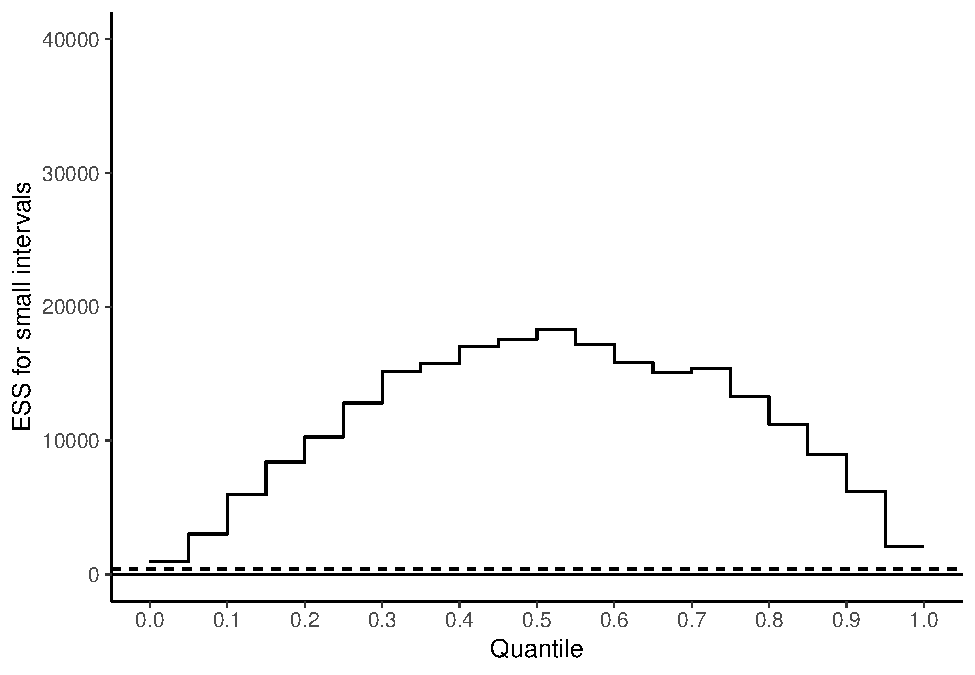
\includegraphics[width=0.98\textwidth]{graphics/local-ess-jags-cp-tau-longer-1.pdf}
  \caption{The local efficiency of small interval probability estimates for 8 schools model with centered parameterization and Gibbs sampling.}
  \label{fig:local-ess-jags-cp-tau-longer-1}
\end{minipage}
\hfill
  \begin{minipage}{0.48\textwidth}
  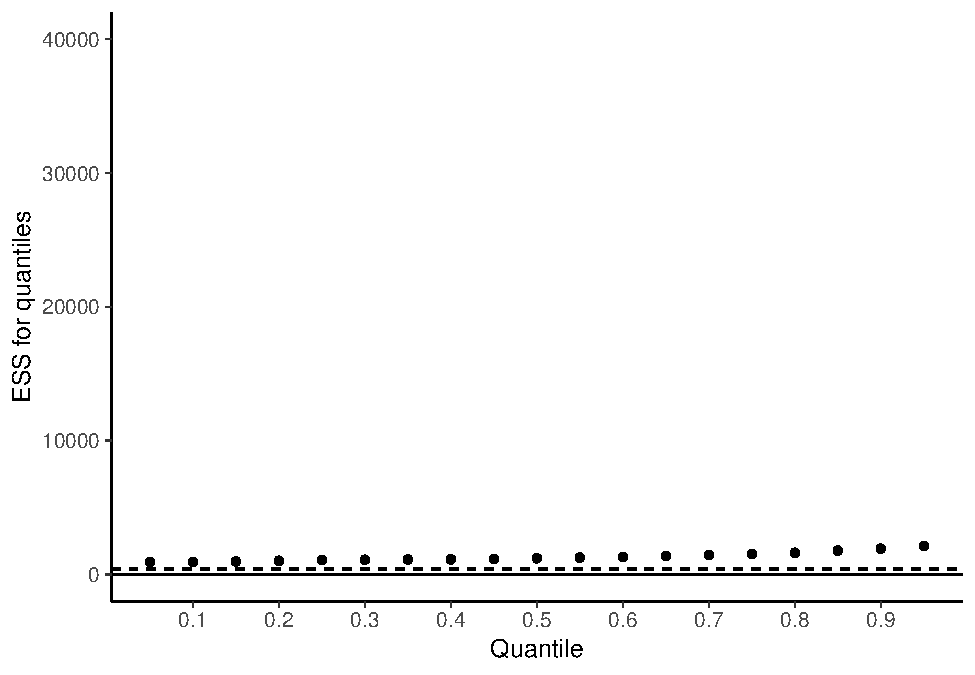
\includegraphics[width=0.98\textwidth]{graphics/quantile-ess-jags-cp-tau-longer-1.pdf}
  \caption{The efficiency of quantile estimates for 8 schools model with centered parameterization and Gibbs sampling.}
  \label{fig:quantile-ess-jags-cp-tau-longer-1}
\end{minipage}
\end{figure}
\begin{figure}[tp]
  \centering
  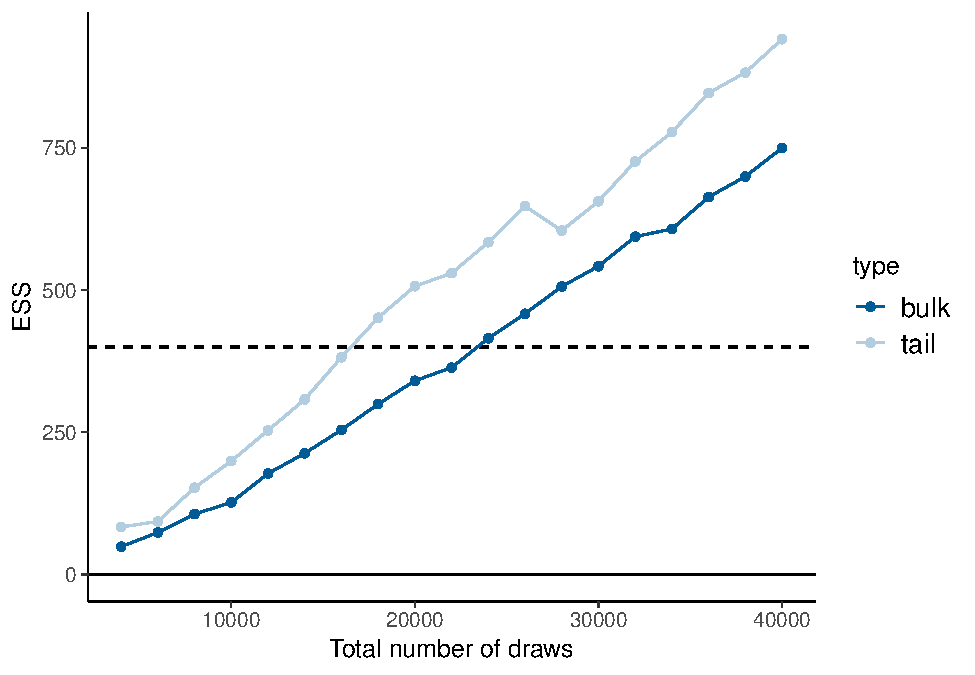
\includegraphics[width=0.47\textwidth]{graphics/change-ess-jags-cp-tau-longer-1.pdf}
  \caption{Rank plots of posterior draws from four chains for 8
    schools model with centered parameterization and Gibbs sampling.}
  \label{fig:change-ess-jags-cp-tau-longer-1}
\end{figure}


\end{document}
